%%%%%%%%%%%%%%%%%%%%%%%%%%%%%%%%%%%%%%%%%
% Short Sectioned Assignment
% LaTeX Template
% Version 1.0 (5/5/12)
%
% This template has been downloaded from:
% http://www.LaTeXTemplates.com
%
% Original author:
% Frits Wenneker (http://www.howtotex.com)
%
% License:
% CC BY-NC-SA 3.0 (http://creativecommons.org/licenses/by-nc-sa/3.0/)
%
%%%%%%%%%%%%%%%%%%%%%%%%%%%%%%%%%%%%%%%%%

%----------------------------------------------------------------------------------------
%	PACKAGES AND OTHER DOCUMENT CONFIGURATIONS
%----------------------------------------------------------------------------------------

\documentclass[paper=a4, fontsize=11pt]{scrartcl} % A4 paper and 11pt font size

\usepackage[T1]{fontenc} % Use 8-bit encoding that has 256 glyphs
\usepackage[ngerman]{babel}
\usepackage{fourier} % Use the Adobe Utopia font for the document - comment this line to return to the LaTeX default
\usepackage{amsmath,amsfonts,amsthm} % Math packages
\usepackage{graphicx}
\usepackage[utf8]{inputenc}
\usepackage{listings}
\usepackage[section]{placeins}
\usepackage{lipsum} % Used for inserting dummy 'Lorem ipsum' text into the template
\usepackage{float}
\usepackage{multicol}
\usepackage{algpseudocode}
\usepackage{algorithm}% http://ctan.org/pkg/algorithms
\usepackage{graphicx,wrapfig}

% Algorithmic modifications
\makeatletter
\newcommand{\ALOOP}[1]{\ALC@it\algorithmicloop\ #1%
  \begin{ALC@loop}}
\newcommand{\ENDALOOP}{\end{ALC@loop}\ALC@it\algorithmicendloop}
\renewcommand{\algorithmicrequire}{\textbf{Input:}}
\renewcommand{\algorithmicensure}{\textbf{Output:}}
\newcommand{\algorithmicbreak}{\textbf{break}}
\newcommand{\BREAK}{\STATE \algorithmicbreak}
\makeatother

\usepackage{sectsty} % Allows customizing section commands
\allsectionsfont{\centering \normalfont\scshape} % Make all sections centered, the default font and small caps

\usepackage{fancyhdr} % Custom headers and footers
\pagestyle{fancyplain} % Makes all pages in the document conform to the custom headers and footers
\fancyhead{} % No page header - if you want one, create it in the same way as the footers below
\fancyfoot[L]{} % Empty left footer
\fancyfoot[C]{} % Empty center footer
\fancyfoot[R]{\thepage} % Page numbering for right footer
\renewcommand{\headrulewidth}{0pt} % Remove header underlines
\renewcommand{\footrulewidth}{0pt} % Remove footer underlines
\setlength{\headheight}{13.6pt} % Customize the height of the header

\usepackage{enumitem}
\setlistdepth{20}
\renewlist{itemize}{itemize}{20}

% initially, use dots for all levels
\setlist[itemize]{label=$\cdot$}

% customize the first 3 levels
\setlist[itemize,1]{label=\textbullet}
\setlist[itemize,2]{label=--}
\setlist[itemize,3]{label=*}

\numberwithin{equation}{section} % Number equations within sections (i.e. 1.1, 1.2, 2.1, 2.2 instead of 1, 2, 3, 4)
\numberwithin{figure}{section} % Number figures within sections (i.e. 1.1, 1.2, 2.1, 2.2 instead of 1, 2, 3, 4)
\numberwithin{table}{section} % Number tables within sections (i.e. 1.1, 1.2, 2.1, 2.2 instead of 1, 2, 3, 4)

\setlength\parindent{0pt} % Removes all indentation from paragraphs - comment this line for an assignment with lots of text

\DeclareMathOperator*{\argmin}{arg\,min}

%----------------------------------------------------------------------------------------
%	TITLE SECTION
%----------------------------------------------------------------------------------------

\newcommand{\horrule}[1]{\rule{\linewidth}{#1}} % Create horizontal rule command with 1 argument of height

\title{
\normalfont \normalsize
\textsc{Karlsruher Insitut für Technologie} \\ [25pt] % Your university, school and/or department name(s)
\horrule{0.5pt} \\[0.4cm] % Thin top horizontal rule
\huge Softwaretechnik II\\ Zusammenfassung WS17/18 % The assignment title
\horrule{2pt} \\[0.5cm] % Thick bottom horizontal rule
}

\author{Manuel Lang} % Your name

\date{\normalsize\today} % Today's date or a custom date

\begin{document}

\maketitle % Print the title
%\newpage
\tableofcontents
\newpage

\section{Vorgehensmodelle}

Vorteile strukturierter Vorgehensmodelle
\begin{itemize}
  \item Reproduzierbarkeit (Erfahrungen für ähnliche Projekte)
  \item Skalierbarkeit (größere Komplexität schneller)
  \item Wiederverwendbarkeit (Code)
  \item Risikominimierung (Entiwcklung nach Plan)
\end{itemize}

Modelle
\begin{itemize}
  \item Softwareentwicklung liefert nicht nur Code, sondern auch Deployment-Deskriptoren (Zusazudokumente), ursprüngliche Anforderungen (Code -> Anforderungen funktioniert nicht), welche Produkte wann und wo?
  \item Wasserfall-Modell\\
    \begin{itemize}
      \begin{minipage}{.5\textwidth}
        \item Erstes Modell zur Definition der verschiedenen Phasen
        \item überhaupt machbar?
        \item Welche Stakeholder?
        \item Lastenheft/Pflichtenheft
        \item Problem: sehr steife Reihenfolge, klingt logisch, aber Phasenübergang ist in Realität unklar
      \end{minipage}
      \begin{minipage}{.5\textwidth}
        \centering
        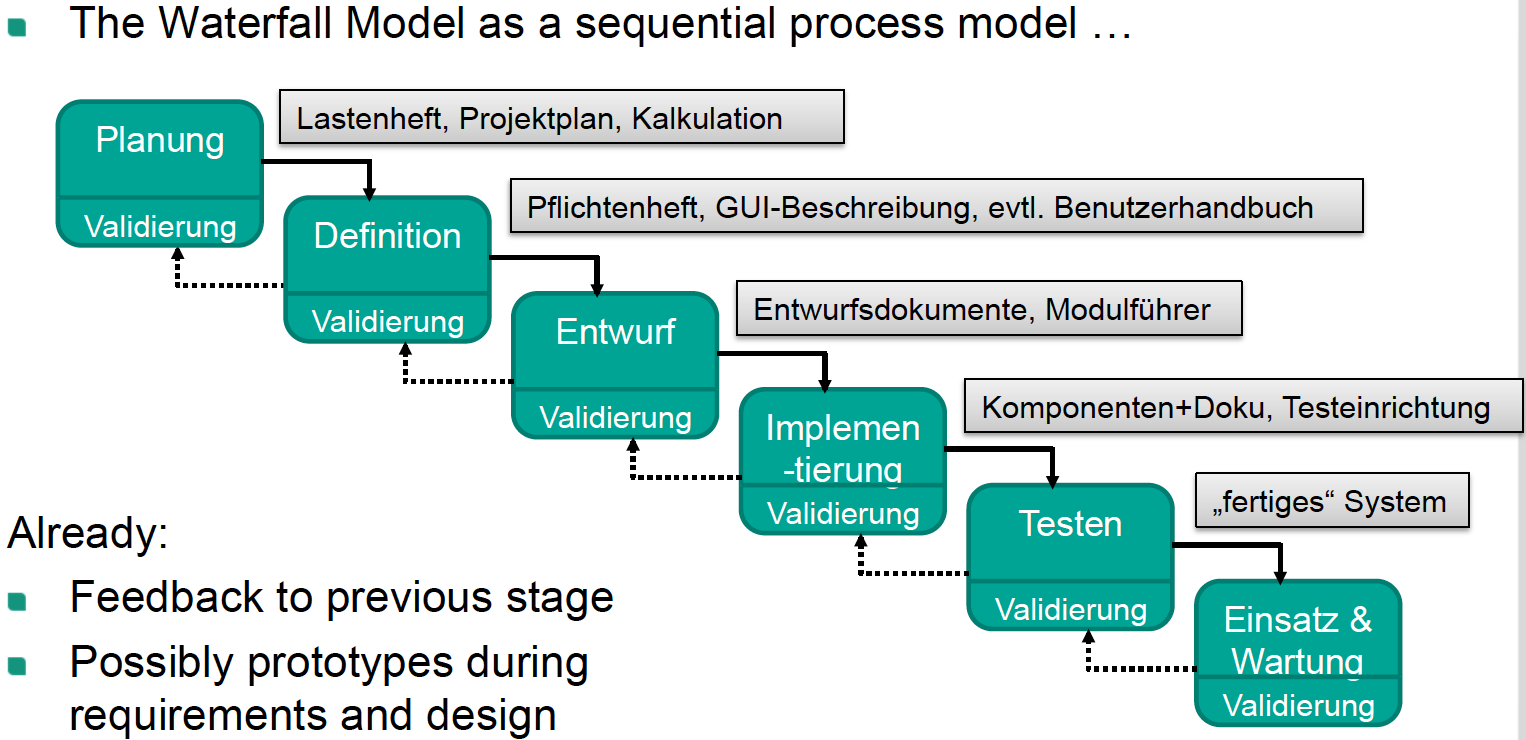
\includegraphics[width=\linewidth]{imgs/wasserfall}
      \end{minipage}%
      \item Feedbackzyklen nötig, aber Unterscheidbarkeit der Phasen trotzdem schwierig
      \item Zu langes Vorplanen (Airbus 10 Jahre?!) sehr schwierig, Was kann in der Zwischenzeit passieren? Niemand weiß das, daher kann Wasserfall langfristig nicht geplant werden (lange Planbarkeit nur sehr selten gegeben)
    \end{itemize}
  \item V-Modell\\
  \begin{itemize}
    \begin{minipage}{.5\textwidth}
      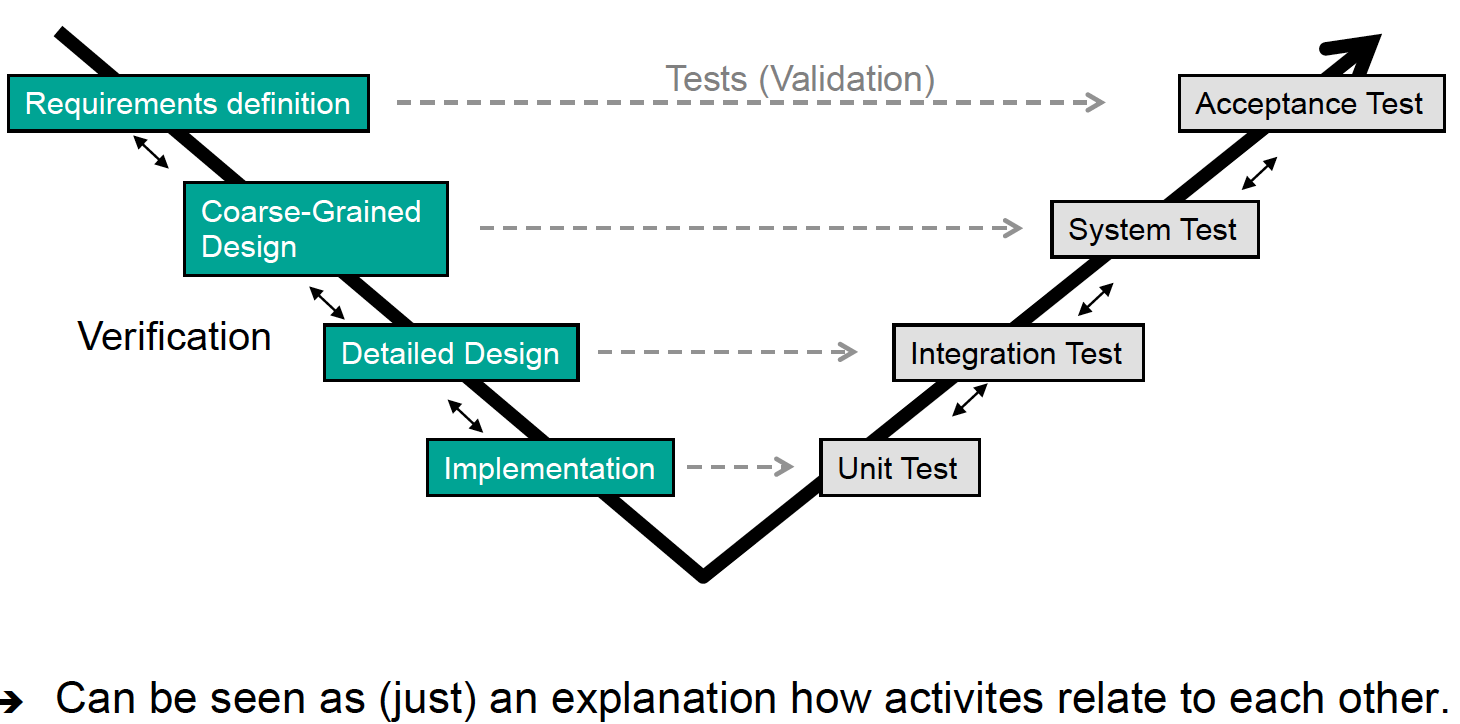
\includegraphics[width=\linewidth]{imgs/vmodell}
    \end{minipage}
    \begin{minipage}{.5\textwidth}
      \item sieht ähnlich aus wie Wasserfall
      \item besagt welche Artefakte man hat + erklärt Zusammenhänge zwischen Dokumenten
      \item überprüft bspw. Zusammenhang zwischen Implementierung und Design (Verifikation, zeigt Abwesenheit von Fehlern, All-Quantor funktioniert immer)
      \item Z.B. mehrere Module zusammen testen (Validierung, nicht Verifikation, Existenz-Quantor, Test-Fall der funktioniert)
      \item Hauptbotschaft: kein notwendiger Wasserfall: Artefakte + Zusammenhänge (Validierung + Verifikation)
    \end{minipage}
  \end{itemize}
  \item 6 grundlegende Phasen in jedem SE-Projekt
  \begin{itemize}
    \item Planung
    \item Definition
    \item Design/Entwurf
    \item Implementierung
    \item Testen
    \item Betrieb
    \item Wartung
  \end{itemize}
  \item 3 Dinge über die ein SE-Modell Aussagen trifft
  \begin{itemize}
    \item Welche Rollen?
    \item Welche Aktivitäten?
    \item Welche Produkte?
  \end{itemize}
  \item Probleme des Wasserfall-Modells
  \begin{itemize}
    \item Sehr lange Zeiträume
    \item inflexibel (schlecht auf Änderungen reagierbar)
  \end{itemize}
  \item Alternativen?
  \begin{itemize}
    \item Inkrementeller Ansatz (nicht zwangsweise flexibel bei geänderten Anforderungen, sondern große Komplexität: mehrere Zyklen für kleinere Teilprojekte), viele kleine kürzere Wasserfälle
    \item Evolutionär: Bei "Fertigstellung" zurückspringen z.B. in Planungsphase, in der Praxis fast immer da z.B. langzeitig Änderungsbedarf auftritt
    \item Gesamtsystem wird nach und nach gebaut
    \item Integrationstests, immer neue Inkremente für Kunden für schnelles Feedback
    \item Konzepte der agilen Entwicklung schon älter
  \end{itemize}
  \item Spiralmodell
  \begin{itemize}
    \item Idee: 4 Quadranten, Zielfestlegung, Bewertung, Validierung, Planung, immer im Kreis um Irrglauben Software ist irgendwann fertig auszuräumen
    \item Nicht inkrementell, sondern evolutionär
  \end{itemize}
  \item UP (Unified Process)\\
  \begin{itemize}
    \begin{minipage}{.5\textwidth}
      \item zuerst UML: vereinheitlichte Notation, z.B. Symbole für Widerstände und Transistoren, Industriestandard
      \item Folge: vereinheitlichte Prozesse, also UP, aber komplett verschieden zu UML (einheitlich), aber es gibt nicht den einen richtigen Software-Prozess, hängt von vielen verschiedenen Faktoren ab (z.B. eingebettete Software), also Rahmenwerk für Prozesse
      \item Verschiedene Phasen: Inception, Elaboration, Konstruktion, Transition über Zeitachse
    \end{minipage}
    \begin{minipage}{.5\textwidth}
      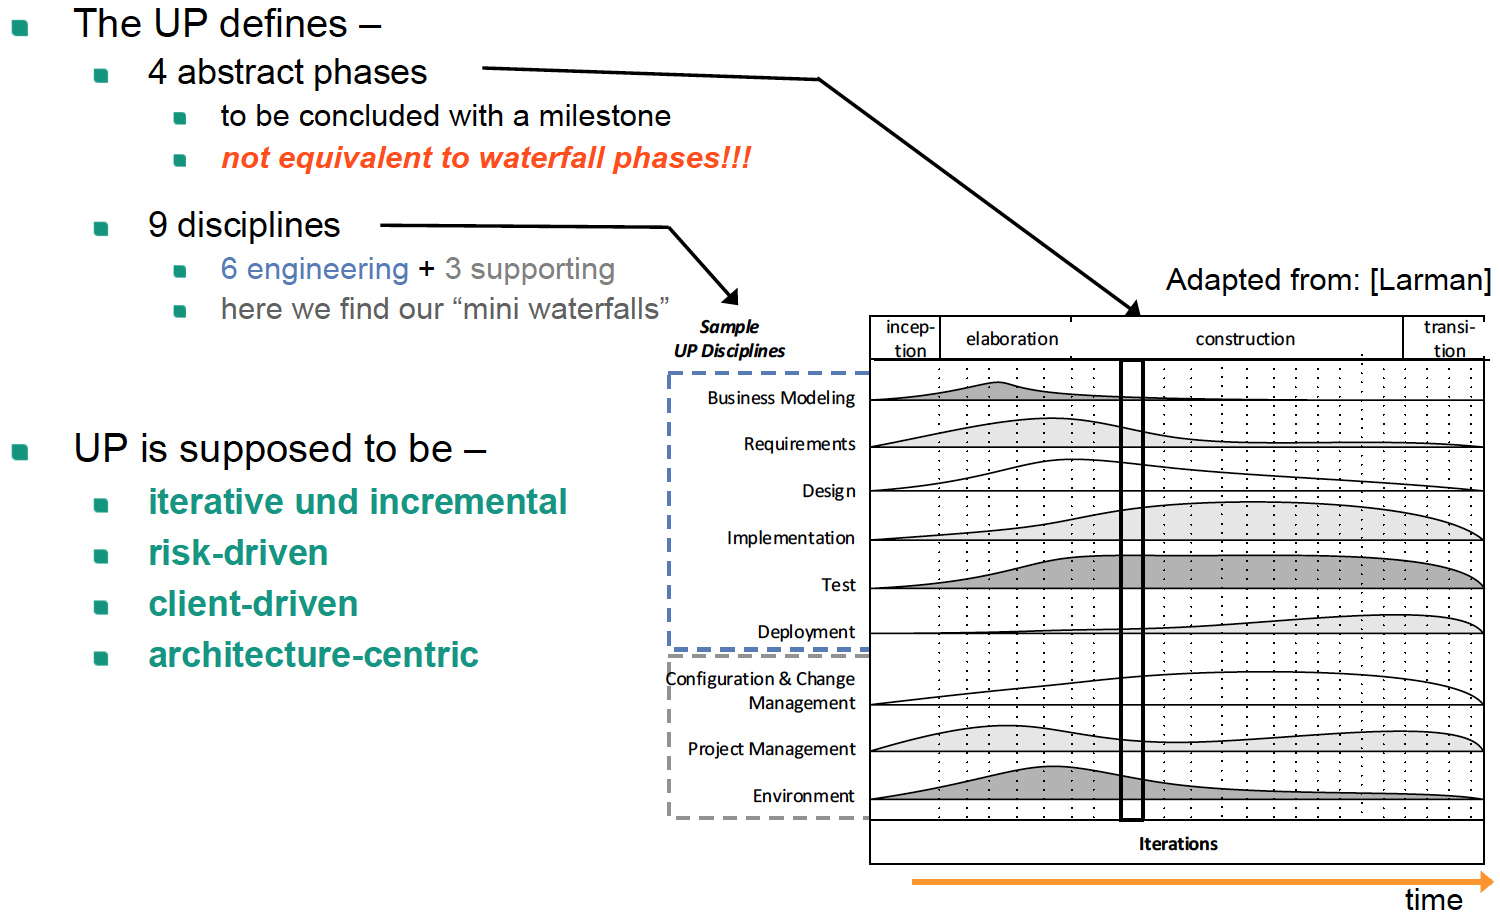
\includegraphics[width=\linewidth]{imgs/up}
    \end{minipage}
    \item Verschiedene Disziplinen wie früher Phasen, auch mit Deployment, insgesamt moderner, andere Disziplinen wie Änderungsmanagement, Projektmanagement, Environment (Entwicklungsumgebung) = Aufrechterhalten der Produktivumgebung + Zusammenspiel der Komponenten + Patches
    \item iterativ und inkrementell (streng nicht dasselbe, iterativ mehrere Schleifen durch Prozess, inkrementell heißt neues Teil), quasi Synonyme
    \item Risiko-getrieben, sehr früh auf Risiken reagierbar
    \item Client-driven: Was will der Auftraggeber?
    \item Architektur-zentriert: zentrales Dokument wovon andere Aktivitäten abhängen
    \begin{itemize}
      \item Inception (Anfangsphase): Scope, Business cases?, machbar?, auf Markt?, Kostenschätzung (schwierig so früh, also sehr grob)
      \item Elaboration (Ausarbeitung): Besonders risikobehaftete Teile werden zuerst betrachtet, Anforderungen verstehen, Übergang in Konstruktionsphase, klappt gut mit sehr erfahreren Entwicklern die Abstraktionsebenen einfach wechseln können, sonst problematisch
      \item Konstruktionsphase
      \item Übergabephase (Test, Deployment)
    \end{itemize}
    \item Disziplinen
    \begin{itemize}
      \item Business Modelling: Technische Konzepte
      \item Anforderungen: Anforderungsanalyse, Dokumentation
      \item Entwurf: Lösungsorientiert, aber kleine klare Grenze zu Anforderungen, nicht nur zeitlich sondern auch konzeptionell überlappend
      \item keine klaren Definitionen!
    \end{itemize}
  \end{itemize}
  \item Rational Unified Process (RUP)
  \begin{itemize}
    \item 6 best practices (sehr generelle Aussagen): iterativ entwickeln, Anforderungen verwalten, Komponenten verwenden, Software grafisch visualisieren, Softwarequalität prüfen, Änderungen unter Kontrolle haben
    \item Was konkret in welcher Phase wurde definiert, konkrete Aufgaben, konkret welche Artefakte
    \item verschiedene Rollen für verschiedene Disziplinen definiert, Anpassungen für konkrete Projekte
    \item prinzipiell genauere Ausarbeitung des UP
  \end{itemize}
  \item Rollen
  \begin{itemize}
    \item Verantwortung abgekoppelt von Person, Reussner Prof. + Vater + Vorstand
    \item eine Person kann mehrere Rollen annehmen
    \item kann aber zu viel Verschnitt führen (viele stehen rum und einer arbeitet, d.h. Gefahr, dass jeder in seiner Rolle bleibt, aber nicht flexibel ist)
  \end{itemize}
  \item Zusammenfassung
  \begin{itemize}
    \item iterativ
    \item UP: Phasen + Disziplinen
    \item RUP: Aktivitäten, Artefakte, Rollen, Rahmenwerk für Projekte
    \item nicht ein gültiger Prozess
  \end{itemize}
  \item Agile Methoden
  \begin{itemize}
    \item kein Allheilmittel
    \item Manifest für agile Softwareentwicklung: Individuals/Interactions > Prozesse, Software > Doku, Kundenzufriedenheit > Vertragsverhandlungen, Flexibilität > Plan folgen
    \item Ist das tatsächlich nötig oder wird Feindbild aufgebaut? Leichter wogegen als wie besser, daher Kritik dass eh niemand so stur ist
    \item Quintessenz: nicht beliebig planbar (Änderungen kommen immer), kontinuierliche Beobachtungen und schnelles Feedback (bau ich was Kunde will? ist Qualität gut?)
  \end{itemize}
  \item Extreme Programming (XP)
  \begin{itemize}
    \item Programmieren = zentral, alles andere außen rum
    \item innen Entwickler: einfache Entwürfe für aktuelle Anforderung, Realisierung mit Pair Programming (verdoppelt Kosten, nicht immer gerechtfertigt, verbessert Qualität auch nicht besser als andere Review-Formen), testgetriebene Entwicklung (immer testbare Software + i.d.R. besser testbare Schnittstellen), Refactoring (Anpassen des Entwurfs für weitere Anforderungen)
    \item außenrum Team: Continuous Integration (keine großen Aufwände bei Builds), Collective Ownership (jeder für alles verantwortlich, kann aber auch fehlschlagen, daher Gesamtprojektverantwortung), Coding Standard
    \item äußerster Kreis: kleine Releases für schnelles Feedback, Kunden testen mit, Planungsspiele (Aufteilen der Inkremente)
    \begin{minipage}{.5\textwidth}
      \item Kritik: ad-hoc Prozess, schwer replizierbar, schlechte Doku, nicht wiederverwendbare Software, Kunden müssen eingebunden werden (will Kunde das?), vieles nicht wissenschaftlich validiert (z.B. Pair Programming), TDD kann problematisch sein
      \item endet in Praxis oft in Code \& Fix
    \end{minipage}
    \begin{minipage}{.5\textwidth}
      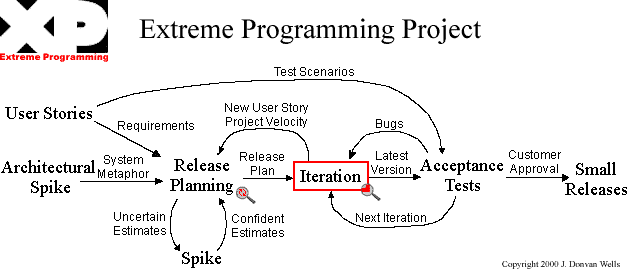
\includegraphics[width=\linewidth]{imgs/XP}
    \end{minipage}
  \end{itemize}
  \item Scrum
  \begin{itemize}
    \item Rahmenwerk mit notwendigen Anpassungen, aber ziemlich elaboriert
    \item Name von Rugby
    \item Product Owner verantwortlich für zu realisierende User Stories und landen als Sammlung in Product Backlog
    \item Inkremente (Sprints): Planning Meeting Product Backlog in Sprint Backlog, Dauer 2-4 Wochen aber konstant
    \item Daily Scrum: täglicher Projektfortschritt, Burn Down Chart (Liste der offenen TODOs abgearbeitet)
    \item Scrum Master trainiert das Team, sorgt dafür, dass sich Entwickler auf das Entwickeln konzentrieren können (also eine stabile Arbeitsumgebung)
    \item Sprint Review Meeting: Wie war die Qualität?
    \item Retroperspective Meeting (Ende vom Projekt): Was hätte man besser machen können? Lehren?
    \item Rollen (pig rolls treiben voran - essentiell): Product Owner (Kundenstellvertreter, vergleichbar mit Architekt), Scrum Master (Hindernisse ausgeräumt, verantwortlich dass Vorgang läuft, damit Entwickler sich auf Rolle konzentrieren können), Team (selbstorganisiert, kümmert sich um Produkt, keine Hierarchie wie bei XP, etwa 7 Leute meist), (chicken rolls - nicht essentiell) Stakeholder, Manager, etc., dürfen Pigs nicht sagen wie sie ihre Arbeit machen
    \item oft TDD
    \item Product Backlog: Sammlung aller Anforderungen, dynamisches Dokument, Priorisierung der Features (z.B. wie stark wird Architektur beeinflusst, wie stark sind Risiken)
    \item Projektplanung: nach jedem Sprint kann etwas ausgeliefert werden, damit schnell Feedback erlangt werden kann, Planung auf 3 Ebenen: Release, Sprint, Arbeitstag
    \item Sprint Backlog: zerbröselter abstrakter Product Backlog für aktuellen Sprint in konkrete Arbeitsaufgabgen, Absprache mit Kunde vlt. nötig, Kategorien: to do, in progress, finished, aber Definition of done?, Sprint Backlog in Product Backlog ist nicht vorgesehen, aber möglich
    \item Sprint Backlog füllen: User Stories vom Product Backlog mit Product Owner und Team Membern diskutiert, oder vielleicht erst Prototyp nötig? Aktivität sollte nicht länger als 2 Tage sein, damit guter Überblick möglich, Abschätzen in Personenstunden, keine Puffer sondern präzise schätzen bspw. durch Time-Box (z.B. 2 Tage nehmen und unter Umständen neu planen)
    \item Wie viel ist genug? Geplant wird weniger, bspw.85\% der Kapazität und zusätzlich etwa 25\% Abzug (Meetings, Urlaub, Krankheit)
    \item Burn Down Chart (Abarbeitung des Product Backlogs über verschiedene Sprints, Infos über Arbeitsgeschwindigkeit zur besseren Planung)
    \item Kritische Bewertung
    \begin{itemize}
      \item Personen/Rollen: Entwickler müssen nahe beisammen sein, kann nur gut klappen wenn sich alle Leute dran halten (benötigt viel Disziplin), effiziente Kommunikation ist wichtig, klappt aber nicht mit vielen Leuten
      \item Artefakte: keine Dokumentation vorgesehen (nur wenn explizit geplant), Code + Testfälle (reicht oft nicht)
      \item Dokumente: -
      \item Aktivitäten: keine Phase zu Architekturentwurf (in Praxis oft Sprint 0 - Architektur)
      \item Skalierbarkeit: sehr schlecht, weil nur für wenig Leute vorgesehen
      \item Architektur: nicht per se vorgesehen
      \item Qualitäts-kritische Software: per se kein Grund wieso nicht agil, aber sehr gute Qualitätssicherung für Sonderfälle sehr wichtig (z.B. Abschaltung Atomkraftwerk), die normalerweise nicht Teil von Scrum sind
      \item große Projekte: Brook's Law (spätes Hinzufügen von Leuten problematisch), daher eher zeitliches Aufsplitten von Team in mehrere Scrum-Teams oder direkt verschiedene Teilteams von Beginn und Scrum of Scrums als Gesamtmeeting
      \item verteilte Entwicklung: Daily Scrum problematisch, Scrum Master immer nah beim Team, Product Owner, wenn sich Leute persönlich kennen auch hier vorteilhaft für Kommunikation, Verteilung während des Projekts kann funktionieren
      \item keine silver bullet, passt bei vielen Projekten, funktioniert aber nicht immer (höchste Qualität, große Gruppen, ...), benötigt viel Arbeit und Disziplin (nicht ad-hoc!), Prozess ansich ist trivial
      \item Distanz zu Code \& fix wichtig
    \end{itemize}
  \end{itemize}
\end{itemize}

\section{Requirements Engineering}

\begin{itemize}
  \item 48\% aller gescheiterten Software Projekte wegen fehlerhaftem RE
  \item IEEE-Standard für Requirement: Fähigkeit die benötigt wird um ein Problem zu lösen
  \item Requirements werden so formuliert, dass...
  \begin{itemize}
    \item prüfbar
    \item präzise (Balance für Entwickler und Auftraggeber)
    \item adäquat (treffen das was Kunde will)
    \item widerspruchsfrei
    \item vollständig (Problem: Wann vollständig?)
    \item risikoabhängig (nicht alles beliebig tief, nur die Dinge die risikobehaftet sind)
    \item eindeutig (adäquat?)
  \end{itemize}
  \item 3 Arten von Anforderungen
  \begin{itemize}
    \item funktional (Features)
    \item nicht-funktional (bspw. Performanz)
    \item Randbedingungen (z.B. gesetzliche Vorgeben oder Platformentscheidungen)
  \end{itemize}
  \item Anfang und Endpunkt der Entwicklung, da Anforderungen auch Akzeptanztests bestimmen, Validierung: hab ich die Anforderungen verstanden? Geänderte Anforderungen ändern auch Akzeptanztests
  \item Requirements Engineering überlappt mit Architekturentwurf, da Rückwirkung auf RE von Architektur
  \item Anekdote über Echtzeit: nicht möglich, da Aufrufe immer anders verzögert, spezielle Hardware + OS nötig
  \item Aktivitäten im RE (iterativ): Eliciation (Was sind die Anforderungen?), Dokumentation (z.B. Use-Cases oder formal z.B. mathematische Verifikation), Übereinstimmung (Widersprüche/Konflikte finden und priorisieren, gemeinsamen Konsens finden), zusätzlich Validieren und Verwalten (Hand in Hand mit anderen Aktivitäten, Änderungen, andere Priosierung)
  \item Stakeholder: Benutzer des Systems (Anwenden), Betreiber des Systems (Deployen), Auftraggeber, Entwickler (und deren Kenntnisse), Architekten (wiederverwendbare Komponenten), Tester (frühe Testbarkeit hilft Validierung der Anforderungen), Botschaft: nicht nur der Anwender
  \item Rolle Requirements Engineer (Anforderungserheber): technisches Wissen ist notwendig, reicht aber nicht, Kommunikation, Konfliktlösung, etc.
  \item Techniken zur Gewinnung von Anforderung: Brainstorming (allein/Gruppe), User Stories zur Kommunikation mit Kunden, Beobachtungen (über die Schulter schauen), Fragebögen, Interviews, Vorgängersysteme? Vorschlagen von Ideen ggü. Kunde sinnvoll
  \item Funktional vs nicht-funktional vs constraint (Kind)
  \begin{itemize}
    \item Verhalten von Software spezifizierbar (Turing Maschine): funktional, sonst nicht-funktional (Wartbarkeit, Sicherheit, Performanz, etc.)
    \item System-Anforderungen (in dieser Vorlesung), sonst Projekt, Prozess
    \item funktional: Funktionalität, System-Verhalten, Daten, ...
    \item nicht-funktional: Performanz, Zuverlässigkeit, Usability
    \item Rahmenbedingung: physisch, Gesetzt, etc.
  \end{itemize}
  \item Andere Facetten
  \begin{itemize}
    \item Satisfaction: Hard/Soft (need vs nice-to-have)
    \item Role: Prescriptive - Wie soll das System sein - vorgeschrieben, Normativ - Umgebung des Systems, Assumptive - Annahme wie mit dem System interagiert wird
    \item Repräsentation: Operational - Spezifikation der Daten, quantifizierbar - messbar, qualitativ - Ziele, deklarativ - rein beschreibend aber kein Umsetzungsgrad
  \end{itemize}
  \item Klassifikationszusammenfassung
  \begin{itemize}
    \item funktional oder nicht-funktional hat nichts mit Repräsentation zu tun
    \item werden in natürlicher Sprache gegeben
    \item Guidelines: kurze Sätze (1 Anforderung pro Satz), klare Formulierung, klar machen wer zuständig ist, schwache Sachen vermeiden (effektiv, Nutzer-freundlich... unprüfbar), Glossar hilft (aber nicht als Selbstzweck), aktive Sprache (Akteure?)
  \end{itemize}
  \item Schablonen verwenden: z.B. The system must/should/will <whom?> <objects> <process word>, Wortwiederholungen nicht wie normal vermeiden, bewusst das selbe gemeint klarmachen!
  \item Natürliche Sprache bietet Vorteile, da sie von allen Stakeholdern verstanden wird, Diagramme o.ä. dagegen nicht unbedingt
  \item Featurelisten: Requirements mit eindeutiger ID um verfolgbar zu sein, verwendbar für Entwurfsentscheidungen, Nachteil: unterschiedliches Abstraktionsniveau und manchmal Liste viel zu feingranular
  \item heutzutage User Stories (agil) oder Use Cases (modellbasiert)
  \item Validierung von Anforderungen: Baue ich das richtige System?
  \item Verifikation von Anforderungen: Baue ich das System richtig?
  \item keine formalen Modelle zur Verifikation
  \item Code Review: gemeinsames Fehlerfinden (Inspektion, Review, Walkthrough)
  \item Simulation: Performance-Eigenschaften simulieren
  \item Prototyping: Mock-Up die Interaktion mit dem System zeigt
  \item Aufstellen von System-Testfällen (zeigt ob Anforderungen verstanden wurden)
  \item Model Checking: formale Verifikationstechniken zum Untersuchen von Widersprüchen
  \item Wie weit RE? Fehlerbehebungskosten? Verweildauer von Bugs? Was sind Kosten einen Fehler zu entfernen ggü. Anforderung zu spezifizieren - 2 Kurven ergeben Wirtschaftlichkeit und Optimum dieser?
  \item Zusammenfassung: Was sind Anforderungen? Wie klassifizieren? Wie aufschreiben? Validierung? Kosten und Vorteile von RE
  \item{Use Cases}
  \begin{itemize}
    \item Helfen geeignete Abstraktionsebene zu finden (auch durch Übung)
    \item Art wie man Anforderungen aufschreibt
    \item Use-Cases nur eine Notation!
    \item Use-Case-Diagramm zeigt Beziehungen der Use-Cases
    \item System oft als Blackbox (also nur Angaben über Schnittstelle)
    \item UI wird in Use Case nicht beschrieben
    \item aus der Sicht der Ziele eines Benutzers
    \item System Boundary: Was wird entwickelt, was nicht?
    \item System Kontext: Gesamte Umgebung die notwendig ist
    \item Context Boundary: trennt System Kontext von irrelevanter Umgebung
    \item Common Scopes: Business use case (Unternehmen ist Blackbox/Whitebox), System use case (System ist Blackbox/Whitebox), component use case (immer Whitebox)
    \item Use Cases als Vorlage für Sequenzdiagramm
    \item Elementary Business Process (EBP): Beschreibung wie Abläufe in Unternehmen funktionieren
    \item Heuristiken: Boss Test (Vorstellung: Chef fragt was habe ich den ganzen Tag gemacht? z.B. Kundenkonten angelegt statt Felder ausgefüllt), Coffee Break Test (logischer Block zu Ende und dann Kaffee trinken), Größe Test (nur 1 Schritt zu wenig)
    \item Verschiedene Ebenen: Summary - gesamter Geschäftsprozess, Ziele eines Benutzers - hier, Subfunktionen - wiederverwendbar in verschiedenen Use-Cases z.B. Anmeldung, Too low - Systemaufrufe
  \end{itemize}
  \item Use Case Diagramm
  \begin{itemize}
    \item Überblick über die Use-Cases
    \item Definieren Use-Cases nicht
    \item Systemgrenzen werden gezeigt
    \item Üblicherweise User Goal Use-Cases (nicht zwangsweise)
    \item Aktoren üblicherweise links
    \item Stakeholder beeinflusst/Bezug
    \item Primary Aktoren lösen Interaktionen aus
    \item Szenario: kann unterschieden werden zu Use-Case (z.B. PIN eingeben), also Instanz eines Use-Cases (z.B. 2x vertippt ... PIN ... etc.)
    \item Wie Use-Cases finden? Systemgrenzen?, Primary Actors?, Welche Ziele (user goals) hat Aktor?, Welche Interaktion braucht man?
    \item Beziehung zwischen Ziel und Szenario? Abhängigkeiten in beide Richtungen, z.B. Szenarien ergeben dass Ziele verfeinert werden müssen, bspw. durch Subziele, zyklische Abhängigkeiten
    \item Iterativer Prozess zur Findung von Use Cases, lieber erst mal Überblick in breiter Suche bevor man zu weit in Tiefe geht, mit viel Erfahrung kann Abstraktionsebene schnell gewechselt werden
    \item Use Case Definition: Aktor, Erfolgsszenario, Wann kein Erfolg? (Bedingungen), Welche Fehler können sinnvoll behoben werden
    \item Aufsplitten oder Zusammenführen kann möglich sein
    \item Use Case Schablonen, bekanntester "fully dressed": Context of us, scope, goal level, primary actor, stakeholder, pre- und post conditions, trigger, main success scenario, extensions, special requirements, technology and data variation lists
    \item Casual: verkürzt
    \item RUP: nahe zu Fully Dressed
    \item Wie Daten beschreiben? Level 1 Data nickname, z.B. PIN, reicht meist, sonst weiter als Typ oder noch weiter mit Länge und Validierung, möglichst keine If-Abfragen, eher trennen
    \item Fully Dressed Use Case sections
    \begin{itemize}
      \item Vorspann bei fully dressed: Actor, Scope
      \item Stakeholder und interessierte
      \item Vorbedingungen: Annahmen über Systemzustand modellieren (sinnvoll, z.B. nicht Stromversorgung)
      \item Nachbedingung: Erfolgsgarantie
      \item Main Success Scenario: keine Verzweigungen
      \item Erweiterung / Alternativen: bei Fehlern (genaues Handling nicht zwangsweise)
      \item Annahmen über nichtfunktionale Anforderungen (z.b. Performanz)
      \item Technologie und Daten
    \end{itemize}
    \item Struktur von Requirements-Dokumenten
    \begin{itemize}
      \item Einleitung (Kontext des Systems, Warum will man das System bauen? Extrem wichtig für Moral/Motivation, Lücken von Spezifikationen können evtl. umgangen werden)
      \item Beschreibung des Systems: Umgebung, Architekturbeschreibung
      \item Anforderungen
      \item Anhang
      \item Index
      \item Beispiel: RUP
      \item versioniert
    \end{itemize}
    \item Werkzeuge für Requirements
    \begin{itemize}
      \item damit nicht bspw. per Email geschickt werden
      \item z.B. ROOM
      \item Multi-user-access
      \item Web-Frontend
      \item Wiki kann auch gut sein (können viele lesen / bearbeiten, billig, aber wenig Generierungsfähigkeit, verschiedene Zugangslevel auch nicht möglich)
    \end{itemize}
    \item Divide and Conquer
    \begin{itemize}
      \item reale Welt
      \item Analyse
      \item Architektur/Design
      \item Code
    \end{itemize}
    \item Zusammenfassung: verschiedene Abstraktionsebenen (summary, user goal), Scopes (business, user goal, component)
  \end{itemize}
  \item Analyse und Entwurf hochgradig verzahnt (aber zwei verschiedene Tätigkeiten, Entwurf Gedanken für Losung)
  \item Operation Contracts
  \begin{itemize}
    \item Anforderungen zu Sequenzdiagrammen / Entwurf?
    \item Input aus Domänenmodell und Use Cases
    \item Sequenz- und Klassendiagramme ableitbar
    \item Design by contract: zwischen zwei Entitäten, aufrufender Kontext und Funktion, Contract für Methode sagt Vor- und Nachbedingung für Objekte und Rückgabewerte
    \item Beschreiben Ablauf
    \item Schema: Name der Operation, Referenzen auf Use Cases, Vor- und Nachbedingung
    \item Nutzen in Business Prozessen, Use Cases, System Operationen oder auch bspw. Java Methoden
  \end{itemize}
  \item Contracts vs Use Cases
  \begin{itemize}
    \item Use Cases für Anforderungen
    \item Contracts können zur weiteren Spezifikation erstellt werden, falls Verfeinerung notwendig
  \end{itemize}
  \item Zusammenfassung Contracts: Operationen identifizieren, Vorbedingung und Nachbedingung, üblichster Fehler ist Vergessen von Assoziationen
\end{itemize}

\section{Software Architektur}

\begin{itemize}
  \item zwischen Anforderungen und Code
  \item Entwurfsentscheidungen dokumentieren
  \item bei jedem Projekt anders
  \item viele Entscheidungen können vorbedingt sein
  \item Verteilung wichtig
  \item Einschränkungen des Entwurfsraums (z.B. objektorientierter vs prozeduraler Stil)
  \item Was evolvieren und was nicht? z.B. wartbar für welches Szenario? Was ist änderbar?
  \item Was wird selbst gemacht, was von außen? Was soll wiederverwendbar sein/werden?
  \item Design vs Architektur: Objektorientierung zwingt zu feingranularer Aufteilung, Architektur übersichtlicher (z.B. Komponentendiagramm)
  \item Verschiedene Sichten auf System (Requirements Engineer, Architekt, Operator, Tester, ...)
  \item Architekturbegriff setzt rationalen Planungsentwurf vorraus (laut Reussner)
  \item Grobe Struktur eines Systems
  \item Definition Reussner: Ergebnis einer Menge von Entwurfsentscheidungen und die betreffen die Komponenten und deren Beziehung untereinander und das Deployment
  \item Nicht ein Diagramm für alles, sondern verschiedene Sichten
  \item Ähnliche Sichten können in Viewpoint zusammengefasst werden (deutsch: Perspektive)
  \item Mindestens 3 Sichten werden benötigt: Aussage über Struktur (Komponenten, Abhängigkeiten), Was passierend während Ablauf (dynamisch, Abstraktion über Verhalten, Kommunikation der Komponenten untereinander oder was passiert bei Methodenaufrufen?), Abbildung auf verschiedene Ressourcen (Deployment View Point)
  \item Decision View Point: um auf View Points zu kommen müssen Entwurfsentscheidungen getroffen werden, warum bewusst Entscheidung getroffen
  \item Alternativ Kruchten 4+1 (logical, development, process, physical view und scenarios), verwendet in RUP, UP noch ausführlicher
  \item Komponentendiagramm gibt keine Aussage über Deployment (z.B. Thin Client vs Fat Client)
  \item Sequenzdiagramm Interaktion über Entitäten
  \item Aktivitätsdiagramm: Ablauf innerhalb von Komponenten
  \item Deployment View: Komponenten abbilden auf Ressourcen (3D, kann gestapelt werden)
  \item Vorteile explizit dokumentierter Architektur: Kommunikationsmedium (z.B. Namen für Komponenten), prüfen ob nichtfunktionale Anforderungen eingehalten werden können, Wiederverwendung, Aufwand von kleineren Komponenten leichter schätzbar, andere Faktoren können einbezogen werden
  \item getrieben von nicht-funktionalen Eigenschaften: Performance (sehr wichtig, Skalierbarkeit), Sicherheit (Architektur kann Exploits vorbeugen, auch wenn die meist durch Entwicklungsfehler entstehen), Verfügbarkeit (Überlastet, Abstürze, ...), Wartbarkeit, nicht sequentiell abarbeitbar, daher Architekturmuster
  \item Faktoren die die Architektur beinflussen: Anforderungen (nicht-funktional und Rahmenbedingungen), Wiederverwendbarkeit (Patterns) - von Vergangenheit aber auch dieses Projekt in Zukunft, Convey's Law: Architektur wird auch durch Form der Organisation der Software beeinflusst (Teamgröße, -erfahrung, Arbeit mit anderen Firmen und anderen Kompetenzen), Funktionale Anforderungen können mit jeder beliebigen Architektur realisiert werden
  \item Wiederverwendbarkeit: Referenz-Architektur (Architektur schon vorgegeben - neue Komponenten werden in Architektur eingebettet - nicht alles muss realisiert werden), Produktlinie
  \item Architekturpattern gröber als Designpattern, Designpattern 1-zu-1 Beziehnung zu Problem, Architekturpattern bieten dies nicht, eher Kompromiss mehrerer funktionaler Anforderungen
  \item Terminologie zur Wiederverwendung: konstanter Stil (nicht mischen), Muster kann man mischen, z.B. Übersetzer (Pipeline, Parser)
  \item Architekturpatterns: Schichtung (z.B. ISO/OSI), Enterprise Application Patterns, Domänenmodell, ...
  \item Design Prinzipien
  \begin{itemize}
    \item Separation of concerns: Dinge die nicht zusammengehören entkoppeln, sonst viel Evaluationsdruck, in Praxis oft smart user interfaces (UI + Logik), z.B. MVC
    \item Single Responsibility Prinzip: nur eine Verantwortlichkeit pro Klasse, folgt als Separation of concerns
    \item Information Hiding: Auswirkung von Architekturentscheidungen lokal, kappseln in Modul
    \item Principle of Least Knowledge (Law of Demeter): keine Annahmen über Entwurfsentscheidungen (z.B. nicht annehmen dass ein Auto einen Motor hat - auto.motor.anlassen() vermeiden, besser: auto.starten() ruft motor.anlassen() auf)
    \item Vermeidung von Redundanzen
    \item (YAGNI) - überleg ob du es brauchst? nicht alle Szenarien planen, Refactoring wenn nötig
  \end{itemize}
  \item Observer Pattern
  \begin{itemize}
    \item löst Problem von verschiedenen Sichten
    \item z.B. verschiedene Sichten auf Datenbestand
    \item Objekt zu beobachten
    \item Beobachter
    \item kann auch als Architekturpattern verwendet werden
  \end{itemize}
  \item Model View Controller \& Observer
  \begin{itemize}
    \item Erweiterung des Observers
    \item Controller und View an Observer, aktualisieren Model
    \item Model aus Domänenebene
    \item verschiedene Realisierungen, z.B. alle Kommunikation muss über Controller oder darf es direkte Kommunikation zwischen View und Model geben?
    \item Applikation (App Controller ist nicht Controller, sondern Aufrufen von Domänenobjekten)
    \item Pro Use Case einen Controller der diesen steuert (häufig als Fassade realisiert) als Daumenregel
    \item bei kleinen Systemen kann Controller auch übersprungen werden
    \item Fassaden: Ein Objekt, dass Zugriff auf andere Objekte steuert, ohne dass genaue Implementierung des zu steuernden Objekts bekannt sein muss
    \item Daten Transfer Objekte: Sammlung von Objekten zusammengefasst
    \item Domain Layer: Domänenmodel, Datenmodell + Funktionalitäten, Übernahme aus objektorientierter Analse
  \end{itemize}
  \item Layered Architecture
  \begin{itemize}
    \item oben User Interface
    \item Geschäftslogik (Anwendungslogik + fachliche Domäne)
    \item unten Infrastruktur
    \item neue User Interfaces entkoppelt (Schnittstellen)
    \item Evaluation schwierig bei neuen Features (Änderung auf jeder Schicht)
  \end{itemize}
  \item Referenzarchitektur hängt mit Layering zusammen, z.B. wird ISO/OSI auch geschichtet (7 Schichten)
  \item Software Komponenten
  \begin{itemize}
    \item Definition: ein Baustein, der komponiert und adaptiert werden kann ohne dass die Innereien verstanden werden müssen. Man wird nicht gezwungen den Source-Code zu lesen bzw. zu verstehen, Widerspruch zu Vererbung (B müsste A kennen um sinnvoll zu überschreiben/erweitern, A weiß nicht ob B seine Methoden überschrieben hat)
    \item Komponenten in Java? kein solcher Begriff "component", Schnittstelle kann implementiert (implements) werden aber Abhängigkeiten nach außen? Daher Dependancy Injection (required-Schnittstelle)
  \end{itemize}
  \item Komponentenmodell
  \begin{itemize}
    \item definiert: was ist eine Komponente? Welche Dienste werden angeboten? Wie werden Dienste angeboten? Wie wird kommuniziert? Beispiel Lego: Platform, Komponentenframework = Noppen (was passt drauf?), Komponenten = Bausteine, Repository = Bestand, Support Tool z.B. Stuhl
    \item technische Realisierungen von CBSE: OMG way - CORBA Framework (Interfacebschreibungssprache zur Generierung von Proxy-Objekten), Sun way - Java, JavaBeans, EJB, Microsoft - .NET CLR, Probleme: Ansätze sind meisten objektorientiert statt komponentenbasiert, daher OSGi?
    \item OSGi: Komponenteneigenschaft, Bundling von feingranularen Objekten, Lebenszyklusmodell
    \item Web Services: sind in einem gewissen Sinne Komponenten, aber Komponenten sind Softwarebausteine, Services können hiearchisch verschalten werden, laufen aber ab (daher Ergebnis kommt zurück, aber kein Baustein)
    \item Software-Oriented Architecture (SOA): Service ist schon deployed, also deployte Komponete
    \item SOFA (Software Appliance): definierte Schnittstelle, Komponente eingesteckt und läuft
    \item ROBOCOP: eigene Infrastruktur
    \item KobrA: architekturorientiert, UML-basiert
    \item Palladio: Architekturen können auch simuliert werden - nicht nur modelliert, Performanzvorhersage zur Design-Zeit, Unterstützung von CBSE, Zuverlässigkeitsvorhersagen
    \begin{itemize}
      \item Palladio Component Model (PCM) ist Sprache um Komponenten zu beschreiben (domain specific modelling language (DSL))
      \item Performancevorhersage: Architekturdiagramm (Modell der Software) liefert durch Simulation Vorhersage für Zeitverhalten (für nicht-echtzeitfähige Systeme)
      \item Was beeinflusst Performance und Zuverlässigkeit einer Komponente? Algorithmus / Implementierung, System Umgebung (Hardware, OS), extern aufgerufene Dienste (z.B. Cloud-Dienste), aber auch Nutzerverhalten (z.B. Dateigröße bei Upload), drei der vier Faktoren kontext-abhängig (nicht von Komponente abhängig), werden alle in Palladio explizit modelliert
      \item Allokationskontext: Komponente auf Umgebung abgebildet (Deployment)
      \item Usage Kontext: Anwendungsprofil, Art der Anwendung der Komponente
      \item Assembly Kontext: Verdrahtung mit extern angeschlossenen Komponenten
      \item Simulator: Änderung der 3 Parameter, z.B. Änderung der Hardware (Allokation) zeigt Änderung der Performance, wie skaliert Sofrware mit mehr Anwendern (Usage)? Was bewirkt veränderte Architektur (Assembly)?
      \item Wieso nicht einfach Prototyp messen? Nachteil: Kosten durch Programmierung, Umgebung benötigt, Deployment auch aufwendig, kann paar hundert tausend Euro kosten, Simulation schneller als Echtzeit, Hardware / Treiber / Last etc. vielleicht nicht verfügbar
      \item Was benötigt man um Performance vorhersagen? Komponentenmodell, Struktur, Deployment Modell, Usage Modell
      \item Was bekommt man: Antwortzeit, Ressourcenauslastung, Durchsatz (akkumuliert - wann erreiche ich x\%)
      \item strikt komponentenbasiert: werden auf Rollen abgebilet
      \begin{itemize}
        \item Komponentenentwicklen
        \item Software Architekt
        \item Software Deployer: Abbildung auf Hardware-Ressourcen (häufig auch durch Architekt)
        \item Domainexperte: Interaktion mit Benutzer oder anderen Systemen (nicht Teil der Architektur)
      \end{itemize}
      \item ViewPoints in Palladio: Structural (Komponentenentwickler, Software Architekt), Behavioral (Komponentenentwickler und Software Architekt), Deployment (System Deployer)
      \item Beschreibung des Verhaltens bei Aufruf von Methoden von Komponenten: beschreibt Kontrollfluss, internal actions können sehr kompliziert sein, sind aber kein externer Aufruf (müssen daher nicht weiter modelliert werden)
      \item Service Effect Spezifizierung: SEFF Einflussfaktoren zusammenpacken
      \item Unabhängigkeit von externen Diensten
      \item Parametrisierung über Ressourcenumgebung
      \item Abhängigkeit von Benutzungsprofil (Parameter)
      \item Parameter kombiniert
      \item Komposition von Komponenten: Komponenten zusammenführen in neue (äußere) Komponente
      \item System Komposition: Aufrufe von außen nach innen abgebildet, Schnittstellen nach außen abgeleitet
      \item Delegation Connector (vertikal - verschachtelt) und Assembly Connector (horizontal - verdrahtet)
      \item Systemmodell: Schnittstelle nach außen, komponentenbasierte Architektur, kann Komponenten von verschiedenen Repositories beinhalten, nur als Einheit deploybar
      \item weitere Aufgaben des Softwarearchitekts: baut Architektur, trifft Entwurfsentscheidungen, Performanceanalyse, Feedback vom Deployment, delegiert die Entwicklungsaufgaben
      \item System Deployer: bildet Komponenten ab auf Ressourcen (können auch verschachtelt werden, Ressourcetypen: CPU, Netzwerk, Speicher (HD, RAM - noch nicht in Palladio))
      \item Domänenexperte: beschreibt Interaktion mit System an äußerster Systemschnittstelle, modelliert Anwendungsverhalten, nicht Komponenten, Benutzungsprofil ähnlich zu SEFF, aber kein Bezug auf Ressourcen oder Komponenten des Systems, Eingabeparameter, wie viele Requests?
      \item TODO Folie 56 einfügen
      \item Am Ende bekommt man Wahrscheinlichkeitsverteilung (Response Time - Wahrscheinlichkeit) oder akkumulierte Dichtefunktion (mit welcher Wahrscheinlichkeit bekommt man Antwort innerhalb gewisser Zeit)
      \item Lesson learned: Kontexte, Einflussfaktoren auf Performance, komponentenbasierte Entwicklung, Trennung Architektur- und Komponentenentwicklung, Black Boxes für Komponenten, SEFF und Parametrisierung
    \end{itemize}
  \end{itemize}
\end{itemize}

\section{Enterprise Application Patterns}

\begin{itemize}
  \item überwiegender Teil von Software
  \item Geschäftsprozesse sollen unterstützt werden
  \item Beispiele: Gehaltsabrechnungen, Online-Shops, Patienten-Daten, Nachverfolgung von Sendungen, Leasing-Systemen
  \item Gegenbeispiele: Telekomunnikationssysteme, Textverarbeitungsprogramme, Betriebssysteme, Anlagensteuerungen
  \item Eigenschaften: Daten sehr wichtig und müssen persistiert werden, große Datenmengen, hochgradig nebenläufiger Zugriff auf Daten, unterschiedliche UI-System (mobile, stationär), verschiedene User-Gruppen (Kunden, Personal, ...), hochgradig vernetzt, oft nicht anpassungsfähig, Komplexität meist durch sehr komplexe Systeme, verschiedene Anforderungen (Skalierbarkeit, Wartbarkeit, ...)
  \item Schichten von EA: Front End, Geschäftslogik, Daten (technologiegetrieben), hier hauptsächlich Domäne + Datenbank (kein Front End, da Technologie sehr schnelllebig)
  \item Patterns
  \begin{itemize}
    \item Muster vs Stile: Stile können nicht gemischt werden, schrenken andere Stile aus, Pattern können kombiniert werden
    \item mehrere Muster für individuelle Probleme
    \item Muster können verschiedene Varianten haben und Implementierung muss häufig selbst gemacht werden
    \item Geschäftslogik Patterns
    \begin{itemize}
      \item Datenmodell existiert, wie strukturier ich Logik?
      \item hohe Komplexität, testbar, wartbar, änderbar, ...
      \item Beispiel: Versicherung macht Auszahlung nach Prämie, anders für jedes Versicherungsprodukt, richtiger Algorithmus für Summe
      \item Transaction Script (Muster)
      \begin{itemize}
        \item Was sind Anfragen die aus Benutzerschicht kommen?
        \item Was wird dafür in der Geschäftslogik benötigt?
        \item Skript macht alle dahinterliegenden Schritte
        \item Gemeinsamkeiten rausfaktorisieren
        \item Vorteile: leicht von Entwicklern verständlich, Transaktionsgrenzen leicht verständlich, einfach auf Datenquellen anwendbar
        \item Probleme: skaliert schlecht mit komplexer Logik, oft Code-Duplikate
      \end{itemize}
      \item Domain Model (Muster)
      \begin{itemize}
        \item Kappselung in Klassen
        \item Objekt-orientierter Ansatz
        \item Vorteil: gut mit komplexer Logik, skaliert gut
        \item Nachteile: Objektorientierung kann schwierig für Entwickler sein
      \end{itemize}
      \item Table Module (Muster)
      \begin{itemize}
        \item Funktion gliedern an Daten, möglichst wie Datenbankschema
        \item Welche Geschäftsfunktionalität kann auf Daten ausgeführt werden?
        \item Lösung z.B. über statische Methoden möglich
        \item Implementierung oft vorgegeben z.B. JDBC
      \end{itemize}
      \item Wann verwendet man was? Orientierung nach Komplexität und Aufwand zur Erweiterung (Domainenmodell etwa linear, Transaktionsskript Vorteile bei einfachen Systemen, Table Module skaliert ab gewinner Größe nicht mehr so gut, also Table Module besser als Transaktions Skript (weniger Duplikationen), Transaktions Skript aber nahe an Terminologie des UI und daher guter und einfacher Einstieg an Software)
      \item Komplexität als Entscheidungskriterium
      \item Wie aufwändig ist es Pattern zu realisieren?
      \item Wie gut können Entwickler Objektorientierung?
      \item Wird Table Module von Middle Ware unterstützt?
      \item Web-Shop hat ziemlich verschiedene Vorgänge mit selben Daten, Komplexität kann höher sein, Performance kann beim Domänenmodell leiden, Table Module könnte bequem sein, sonst auch Transaction Script möglich, da Code Duplikation eher unrealistisch scheint
      \item Leasing System kann komplexe Domänenlogik haben, deshalb Domänenlogik
      \item Expense Tracking System muss gut erweiterbar sein, aber nicht so komplex, muss schnell entwickelbar sein, Domänenmodell für Erweiterbarkeit, die anderen können später schwieriger geändert werden, Argument für Transaktionsskript geringer initialier Aufwand
    \end{itemize}
    \item Data Source Architectural Patterns
    \begin{itemize}
      \item Wie stelle ich objektorientiert Daten da, die aus nicht OO-Datenbank kommen
      \item Auch bei NOSQL - muss auch OO Dargestellt werden
      \item Lösungen: Manuell (JDBC), Hibernate (oder andere OR-Mapper) oder XML
      \item Zur Wartbarkeit keine SQL-Statements im Code verstreuen!
      \item Record Set (Muster)
      \begin{itemize}
        \item Daten in einer Tabelle als geordnete Liste im Speicher (in-memory) abgelegt
        \item Eine Klasse des Record Sets mit Tabellen verknüpft
        \item ResultSet im Code mit dem gearbeitet werden kann (z.B. AcetiveX Data Objects oder JDBC)
        \item Zugriff über Strings (resultSet.getString("Fname");) nicht schön, Typfehler erst zur Laufzeit
        \item schlechte Wartbarkeit - ist es wirklich das Set?
      \end{itemize}
      \item Table Data Gateway (Muster)
      \begin{itemize}
        \item Objekt einer Klasse, das Schnittstelle zur Datenbanktabelle ist
        \item Instanz Zugriff auf alle Tabellen
        \item CRUD Operationen durchführbar
        \item Gateway-Klasse implementiert SQL-Statements
        \item beißt sich mit Domänenmodell, da Daten stark nach DB gegliedert, anders als bei Domänenmodell, passt aber gut zu Transaktionsskript
        \item Gateway oder Fasade: Fasade verschattet möglichst komplexe Struktur und bietet einfachen Zugriffsweg, Gateway kappselt bewusst wie auf Datenbank zugegriffen wird, Fasade wird von Entwickler zur Verfügung zur Verfügung stellt, Gateway wird von Nutzer zur Verfügung gestellt
      \end{itemize}
      \item Active Record (Muster)
      \begin{itemize}
        \item Objekt das eine Zeile der Datenbank beinhaltet, Geschäftslogik mit integriert
        \item Passt sehr gut zur Domänenlogik
        \item Gibt kein Record-Set, eine Instanz auf die CRUD-Operationen ausführbar sind
        \item Nachteile: bei komplexerer Geschäftslogik können Funktionen benötigt werden, die auch Zugriff auf andere Objekte benötigen
        \item Klappt nicht bei viel Verarbeitung - wie bei Oberklasse?
        \item sehr stark an Datenbankschema orientiert
      \end{itemize}
      \item Row Data Gateway (Muster)
      \begin{itemize}
        \item Objekt einzelner Zugriff (Zeile), aber ohne Geschäftslogik
        \item Vorteil: mehr Freiheitsgrade zur Strukturierung der Geschäftslogik
        \item Gut für Code Generierung, Entkoppelung von DB
      \end{itemize}
      \item Identity Map (Muster)
      \begin{itemize}
        \item Zugriff auf DB
        \item Überprüfung ob Objekt schon da ist
        \item Nur eine Instanz von Objekt, nicht mehrere Instanzen von "dem selben"
      \end{itemize}
      \item Data Mapper (Muster)
      \begin{itemize}
        \item Schicht die sich darum küppert wie Daten in DB kommen
        \item Entkoppelt durch Mapper
        \item Felder, Arrays geklärt
        \item Übergang von Objekt-Schema und relationes Schema
        \item auch als DAO bekannt
        \item Werkzeuge existieren, Larman: "Don't try this at home!"
        \item OR-Mapper können einiges dieser Funktionalität
        \item Wann verwenden: Legacy Systeme (Datenbestände da, aber System nicht mehr aktuell), Active Record ist nicht mehr ausreichend für Geschäftslogik, Datenbankschema und Objektmodell müssen unabhängig evolviert werden
      \end{itemize}
      \item Wann sollte man was verwenden? Geschäftslogik nach Transaktionslogik, dann Row Data Gateway oder Table Data Gateway (für record set), falls Domänenmodell für einfachen Code Active Record, bei komplexen Mappern Data Mapper, falls Table Module dann Table Data Gateway, Kombinationen möglich (hier eher da unterschiedliche Datenbestände möglich)
    \end{itemize}
    \item Objekt-relationale Patterns
    \begin{itemize}
      \item relationale Datenbank + objekttorientierte Struktur im Business Layer (mit Vererbung)
      \item müssen sehr häufig nicht selbst implementiert werden
      \item Single-Table Inheritance
      \begin{itemize}
        \item alles in eine Tabelle
        \item Vereinigung der Attribute in Tabelle
        \item Namenskonflikte in OOP zu lösen
        \item Vorteile: sehr einfach, keine Joins, Refactoring von Felder hoch und runter benötigt keine Änderungen der Datenbank
        \item Nachteile: wenn irgendwo was geändert wird, muss immer Tabelle geändert werden, Tabelle kann sehr groß werden, für Basisklasse müssen alle Eigenschaften angelegt werden auch wenn diese nicht gebraucht werden
      \end{itemize}
      \item Class Table Inheritance
      \begin{itemize}
        \item Jede Klasse bekommt eigene Tabelle
        \item wieder 1:1 Mapping der Attribute
        \item Vorteile: Felder werden sinnvoll verwendet (keine leeren), konzeptionell sehr einfach
        \item Nachteile: viele Joins (Performanceprobleme möglich), häufiger Zugriff auf Super-Types
      \end{itemize}
      \item Concrete Table Inheritance
      \begin{itemize}
        \item Attribute der Oberklasse werden nach unten mit kopiert (nur nicht abstrakte)
        \item Vorteil: wenger Platzverschwendung, Joins vermieden
        \item Nachteil: Felder werden kopiert, bei Änderung der Oberklasse müssen alle Tabellen geändert werden
      \end{itemize}
      \item Wann nehme ich was? Single Table: eher bei Instanzen der Unterklassen, Performance-Vorteil, Class Table: offensichtliche Struktur, Concrete Table: ohne Joins
    \end{itemize}
  \end{itemize}
  \item Java Persistence API
  \begin{itemize}
    \item viele Muster implementiert
    \item nicht zwangsweise Enterprise JavaBeans (EJB)
    \item O/R Mapping in Hibernate mit \@-Annotationen
    \item Single Table Inheritance als Beispiel
  \end{itemize}
\end{itemize}

\section{Microservices}

\begin{itemize}
  \item keine genaue Definition, aber Eigenschaften: Aufteilung in Services, Design for failure, enger Zusammenhang zur Automatisierung der Infrastruktur (CI/CD) für schnelleres Feedback ermöglicht kleine Inkremente, dezentralisierte unabhängige Komponenten, Produkt mehr im Vordergrund als Projekt
  \item Service ausführbar im Gegensatz zu Komponenten
  \item kompletter Stack wird durchgetrennt, oft mehrere Datenbanken um alles zu entkoppeln
  \item dezentralisierte Verwaltung der einzelnen Säulen
  \item Design for Failure ergibt sich durch Entkopplung (ein Auswahl führt nicht dazu, dass auch andere ausfallen)
  \item Evolution sehr leicht möglich (viele Releases möglich)
  \item Wenn CI/CD wichtig, dann sind Microservices spitze!
  \item aber auch Nachteile: z.B. schnell Redundanzen im Code
  \item Architekturstil (1x MS dann im ganzen Projekten)
\end{itemize}

\section{Objektorientierter Entwurf}

\begin{itemize}
  \item Geschäftslogik organisieren
  \item Wiederverwendung
  \item Funktionen zu Objekten zuweisen
  \item Kriterien: Jemand ist verantwortlich etwas zu tun oder jemand weiß etwas und daraus ergibt sich Verantwortung
  \item Aus Domänenmodell sind Methoden erahnbar
  \item In der agilen Welt häufig als Kommunikationsmittel gedacht
  \item Interaktionsdiagramme wichtig
  \item Design Class Diagram (DCD) - Fragment eines Klassendiagramms, beschreibt eine Klasse (dient zur Übersichtlichkeit bei vielen Klassen)
  \item Klassen identifizieren: auch Klassen aus dem technischen Entwurf die sich nicht aus dem Domänenmodell ergeben
  \item Methoden aus Sequenzdiagramm hinzufügen (Klassen aus Entwurf)
  \item Controller Pattern: Controller kappselt bestimmen Use-Case
  \item Pure Fabrication Pattern: Methode wird zurückgeliefert die nicht im Domänenmodell verfügbar ist (z.B. Data Mapper), gut wenn zu viel Evolutionsdruck auf selbe Klasse
  \item GRAS Patterns (GRASP)
  \begin{itemize}
    \item Creator Pattern
    \begin{itemize}
      \item Ich bin verantwortlich für Erzeugung von X wenn für Objekt C gilt, C contains oder aggregates X (X ist Teil von C), C verwendet X häufig (C ruft viele Aufrufe von X auf) oder C beinhaltet Initialisierungsdaten für X (je mehr desto besser für Pattern)
    \end{itemize}
    \item Controller Pattern
    \begin{itemize}
      \item Grund 1: Zentralle Klasse soll Use-Cases bearbeiten
      \item Composer Component: Fasaden-Muster (Fasaden-Controller) kann Use-Case beinhalten
    \end{itemize}
    \item Low Coupling \& High Cohesion
    \begin{itemize}
      \item Wenn 2 Sachen eng zusammenarbeiten, dann in eine Komponente (hohe Kohesion kappseln und niedrige Kopplung, geringe Kohesion aufsplitten)
      \item Beispiel: Fasade Split (nicht so toll) - Fasaden oft Gott-Klassen
    \end{itemize}
    \item Polymorphie
    \begin{itemize}
      \item z.B. viele verschiedene Payments, dann abstrakte Klasse Payment die Authorisierungs-Methode vorgeben (häufig in Praxis instance of Typabfrage in Hauptklasse - grausam, da nicht neue Unterklassen hinzugefügt werden können und Oberklasse soll nicht Unterklassen kennen)
      \item Vererbung ist Whitebox-Technik, Komposition dagegen Blackbox-Technik (Interna nicht relevant), Beispiel: RubberDuck erbt von Duck, aber Duck definiert fly(), was passiert in Unterklasse - Exception?
      \item Mehrfachvererbung in C++ könnte helfen mehrere Superklassen zu definieren
      \item In Java dagegen Strategiemuster: Ente, Schnittstellen die FlyBehaviour und QuackyBehavior definieren (Komponenten statt Vererbung)
    \end{itemize}
    \item Pure Fabrication
    \begin{itemize}
      \item Datenbankevolution und Geschäftsmodellevolution in selber Klasse
      \item Daher Entity Manager oder PersistentStorage erzeugt Methode zur Datenbankankopplung
    \end{itemize}
    \item Indirection
    \begin{itemize}
      \item Aufgaben werden an andere Klassen delegiert
      \item wegen zu hohem Evolutionsdruck
      \item Pure Fabrication ist Spezialfall von Indirection
    \end{itemize}
    \item Law of Demeter
    \begin{itemize}
      \item Eine Klasse soll nicht zu beliebig anderen Klassen Kontakt haben
      \item Methode soll nur mit Objekten der gleichen Klasse, Methoden der Methode, Attribute ihren Attributen oder in der Methode erzeugten Objekten kommunizieren
    \end{itemize}
    \item Wichtig: Diagramme auf Patterns anpassen, sofern diese nicht von vornherein geplant sind
  \end{itemize}
\end{itemize}

\section{Clean Code}

\begin{itemize}
  \item Es gibt immer Code
  \item Schreibe Code immer für den nächsten Entwickler, nicht für den Compiler / Interpreter
  \item Schlechter Code verringert die Produktivität exponentiell
  \item Lehman's first law: A system that is used will be changed
  \item Lehman's second law: An evolving system increases its complexity unless work is done to reduce it
  \item Der Aufwand der für eine Änderung im System auftritt, erhöht sich je später sie auftritt
  \item Die Kurve kann durch agile und iterative Methoden flach gehalten werden
  \item Was ist "Clean Code"?
  \begin{itemize}
    \item elegant und effizient
    \item offensichtliche Logik
    \item minimale Abhängigkeiten
    \item macht eine Sache gut
    \item einfach und direkt
    \item liest sich wie gut geschriebenes Prosa
    \item verdeckt niemals die Intention des Designers
    \item leicht erweiterbar
    \item Code, um den sich gekümmert wurde
    \item Guter Code: "Weniger WTFs pro Minute"
  \end{itemize}
  \item Objektorientiertes Design
  \begin{itemize}
    \item GRASP aus der vorherigen Vorlesung
    \item Die 5 SOLID Prinzipien
    \begin{itemize}
      \item Single Responsibility Principle (SRP)
      \begin{itemize}
        \item "There should never be more than one reason for a class to change."
        \item Jede Verantwortung behandelt ein Belangen
        \item Schelcht: große Klassen (über 200 LOC, über 15 Methoden/Felder)
        \item Refactoring: Klasse verkleinern
        \item Nutzen: Code leichter verständlich, Hinzufügen oder Modifizieren sollte nur wenig Klassen beeinflussen, Risiko den Code zu zerstören wird minimiert
        \item Einschub - Command-Query-Separation: Aktionen und Aufrufe trennen, damit Nebeneffekte vermieden werden
      \end{itemize}
      \item Open Closed Principle (OCP)
      \begin{itemize}
        \item "Software entities (classes, modules, funktions, etc.) should be open for extensions, but closed for modification"
        \item Verhalten sollte durch neuen Code verändert werden, nicht dadurch alten Code zu ändern
        \item Sehr stark verbunden mit dem "Information Hiding Principle"
      \end{itemize}
      \item Liskov Substitution Principle (LSP)
      \begin{itemize}
        \item Funktionen die Pointer oder Referenzen zu Basis-Klassen verwenden müssen Objekte der Basis-Klasse verwenden können
        \item Verbunden zu Design by Contract: "When redefining a routine [in a derivative], you may only repalce its precondition by a weaker one, and its postcondition by a stronger one."
      \end{itemize}
      \item Interface Segregation Principle (ISP)
      \begin{itemize}
        \item "Clients should not be forced to depend upon intercaes that they do not use."
        \item Steckdosen-Metapher: es kann nur ein Gerät eingesteckt werden
        \item Interfaces sollten so schlank wie möglich gehalten werden, hohe Cohesion - nur ein Konzept, sollten nicht von anderen Interfaces abhängen nur weil eine Unterklasse beide benötigt
        \item getrennt wenn sie von verschiedenen Clients verwendet werden
      \end{itemize}
      \item Dependancy Inversion Principle (DIP)
      \begin{itemize}
        \item "A. High level modules should not depend upon low level modules. Both should depend upon abstractions.
        B. Abstractions should not depend upon details. Details should depend upon abstractions."
        \item Designproblem: Generischen Algorithmus von detailliertem Kontext trennen
        \item Template Method Pattern: Inheritance, Binding zu Compile-Zeit, hängt stark von Algorithmus ab und verletzt DIP
        \item Strategy Pattern: Parametrisierung mit Konstruktor oder Setter
        \item Dependancy Injection: Technologie um abstrakte Abhängigkeiten mit konkreten Objekten zur Laufzeit zu instanziieren
        \item Inversion of Control (IoC) Container
        \item vereinfacht Testen
        \item entkoppelt Boilerplate Code
      \end{itemize}
    \end{itemize}
    \item Law of Demeter ("Don't talk to strangers"): Eine Methode m der Klasse C sollte nur Methoden der Klasse C, von m erstellte Objekte, als Argument an m übergebene Argumente oder Objekte von Instanzvariablen von C aufrufen.
    \item Boy Scout Rule: "Leae the campground cleaner than you found it!" - aufrichtig sein ggü. Code, Kollegen, zu sich selbst, agile Werte (XP, Scrum): Aufräumen ist Teil von Conecpt of Done
    \item Principle of Least Surprise: "Any function or class should implement the behaviours that another programmer could reasonably expect." , wenn offensichtliches Verhalten nicht implementiert wird, können Leser und Anwender nicht ihrer Intuition vertrauen und müssen Internals lesen
    \item Code Conventions
    \begin{itemize}
      \item Naming: standardisiert, aussagekröftig (für jeden klar) - Hinweis über Kontext (AccountName in Account-Klasse), Hinweise über Typen (nameString, accountList), bestimmte prefixes (m\_name, IName), können durch IDE bereitgestellt werden, aussagelose Namen Vermeiden (außer Sonderfälle wie i als Schleifeninvariante)
      \item Kommentare: nicht schlechten Code kommentieren, besser neuschreiben, gute Kommentare sind aussagekräftig (z.B. Test case takes ages), warnend (X used here isn't threadsafe), informativ (TODO: .. Will take care of missing..), aber aussagekräftiger Code ist besser als viele Kommentare
    \end{itemize}
    \item Formatierung: Kohesionslevel visuell repräsentieren, vertikaler Abstand zwischen Konzepten (z.B. nach Imports oder Methoden), horizontaler Abstand um Operatoren oder Parameter zu betonen - verdeutlichen Elemente, häufig unterstützen IDEs Auto-Formatierung
    \item Don't Repeat Yourself (DRY) - copy \& paste reduziert Wartbarkeit, Verständllichkeit und Evolvierbarkeit, Code-Duplikation fördert Fehler und Inkonsistenzen
    \item Keep It Simple, Stupid (KISS) - "Make everything as simple as possible, but not simpler" (Albert Einstein), guter Code ist für jeden leicht verständlich, guter Code adressiert das Problem adäquat, z.B. wenn IEnumerable ausreicht, verwende keine ICollection oder eine IList, Techniken die helfen dass Code für andere verständlich ist: Code Reviews, Pair Programming
    \item You Ain't Gonna Need It (YAGNI): Features sind teuer (+Testen/Dokumentation) und machen das System schlechter wartbar da sie komplex werden (KISS), Vorsicht vor Optimierungen (kann teuer werden)
    \item Single Level of Abstraction (SLA): Abstraktion wie Zeitung - TODO
  \end{itemize}
  \item Clean Architecture Patterns
  \begin{itemize}
    \item verschiedene Designpatterns: heagonale Architektur ("Ports and Adapters", bessere Testbarkeit des Kerns und unabhängig von äußeren Services die leicht ersetzbar sind), Zwiebel Architektur (kontrolliert Coupling, da es richtung Zentrum geht), Boundary/Control/Entity(BCE): Varation des MVC, Verteilung der Verantwortungen
    \item Clean Architecture Patterns führen zu Unabhängigkeit von Frameworks, testbaren Systemen, Unabhängigkeiten vom UI, Unabhängigkeit von Datenbanken, Unabhängkeite von externen Gegebenheiten
    \item "Clean Architecture": kreisförmige Schichten repräsentieren verschiedene Bereich von Software (weiter innen = höheres Level der Software, außen Mechanismen, innen Policies), "The Dependancy Rule": Source Code Abhängigkeiten zeigen immer nach innen
    \item Entities: Kappseln Business Rules, Objekt mit Methoden, Datenstruktset mit Funktionen, kann als Businessobjekt für Anwendungen verwendet werden, operationale Änderungen sollten die Entity nicht ändern
    \item Use Cases: beinhaltet architekturabhängige Business Rules, implementiert Use Cases des Systems, Schicht sollte sich nicht ändern bei Änderung der Entitites oder DB, UI oder anderen Externas, Schichte sollte sich ändern bei operationalen Änderungen der Anwendung
    \item Interface Adapters: Betrifft Datenaustausch zwischen Schichten, beinhaltet MVC Architektur eines GUI, Modelle sind Datenstrukturen
    \item Grenzen überschreiten: Controller und Presenter kommunizieren in Use-Cases, Source Code Abhängigkeiten zeigen nach innen (meist mit Dependancy Inversion)
    \item Refactoring: "If it strinks, change it." (Grandma Beck), Beispiele: Methoden/Klassen extrahieren, Methoden/Felder verschieden, Inline Klassen, ABER: Refactoring nur mit Tests, Bad Smells: lange Methoden, duplizierter Code, Aufruf Methoden anderer Klassen, Datenklassen, riesige Klassen / Gottklasse, ..., Format des Refactorings: Name, Zusammenfassung, Motivation, Mechanismus, Beispiel, Wann refactorn: wenn "Bad Smells" auftauchen, Limitationen: Performance, Persistenz, Interfaces
  \end{itemize}
\item Zusammenfassung: Empfehlungen wie Code zu strukturieren, Refactoring für saubereren Code, Design Philosophien und Prinzipien
\end{itemize}

\section{Model Driven Development}

\begin{itemize}
  \item Was ist ein Modell?
  \begin{itemize}
    \item Abbildungsmerkmal: Modelle sind immer Modell von etwas, d.h. Abbildung von natürlichen oder künstlichen Originalen, die auch Modelle sein können
    \item Verkürzungsmerkmal: Modelle beschreiben nicht alle Atriibute des Originals, nur die als für Ersteller und Anwender wichtig erarchteten
    \item Pragmatisches Merkmal: Modelle sind ihren Originalen nicht eindeutig zugeordnet. Sie erfüllen ihre Substitutionsfunktion a) für bestimmte Subjekte, erkennen oder handeln, mit Hilfe von Modellen, b) in bestimmten Zeitabständen und c) unter Einschränkung auf bestimmte mentale oder tatsächliche Operationen.
    \item Original kann durch eine Vielzahl von Modellen beschrieben werden
  \end{itemize}
  \item Metamodelle (griechisch meta = nach): Modelle die Modellierung beschreiben, beschreibt die Struktur von Modellen (Kontrukte der Modellierungssprache, Assoziationen zwischen Elementen, Constraints, Modeling Rules)
  \item Beschreibung von Metamodellen
  \begin{itemize}
    \item meist in formaler Sprache beschrieben
    \item bisher (VL + Zusammenfassung) nur UML Klassendiagramme
    \item Klassendiagramme verwedendet für modellbasierte Software-Entwicklung und hauptsächlich für Kommunikation designed
    \item Spezifikation von Metamodellen
    \begin{itemize}
      \item Abstrakte Syntax: beschreibt die Konstrukte des Modells und die Eigenschaften und Beziehungen zwischen ihnen, Beschreibung ist unabhängig von der konkreten Darstellung dieser Konstrukte, Eigenschaften und Beziehungen.
      \item Konkrete Syntax: beschreibt die Darstellung von Konstrukten, Eigenschaften und Beziehungen, die in der abstrakten Syntax spezifiziert sind. Für die abstrakte Syntax eines Metamodells muss mindestens eine konkrete Syntax angegeben werden, und beliebig viele können angegeben werden.
      \item Statische Semantik: beschreibt die Modellierungsregeln und -einschränkungen, die in der abstrakten Syntax nicht ausgedrückt werden können. Für die Definition von Restriktionen als Constraints gibt es spezialisierte Sprachen (z.B. OCL).
      \item Dynamische Semantik:beschreibt die Bedeutung seiner Konstrukte. Die dynamische Semantik wird oft nicht formal festgelegt, sondern durch Texte in natürlicher Sprache. Durch die Erstellung eines Mappings des Metamodells auf eine Sprache mit genau definierter Semantik (z.B. Petri-Netze) kann die dynamische Semantik formal spezifiziert werden.
    \end{itemize}
  \end{itemize}
  \item Representation / Instatation
  \begin{itemize}
    \item Modell repräsentiert Original
    \item Wenn das Modell preskriptiv (vor dem Original) erstellt wurde, dann Instanziiert das Original das Modell
    \item Metamodelle werden normalerweise im vorraus erstellt, damit Modelle als Instanzen erstellt werden können
    \item häufig Modellierung in vier Schichten
  \end{itemize}
  \item Selbstbeschreibende Modelle
  \begin{itemize}
    \item Modelle der abstraktesten Schicht werden oft "self-descriptive" genannt
  \end{itemize}
  \item Model-Driven Software Development (MDSD)
  \begin{itemize}
    \item Model-Driven Engineering: Kombination von Domain-specific modelling languages (DSML) - Deklarative Beschreibung der Anwendungsstruktur, Verhalten und Anforderungen, Transformation Motoren und Generatoren, Ziel: Reduktion der Plattform Komplexität
    \item Model-Driven Software Development: Anwendung von MDE für Software-Entwicklung, andere Anwendungen: Hardware-Entwicklung, Software-intensive Systeme, Laufzeit-Modellierung
    \item Model-Driven Architecture: Markenzeichen der Object Management Group (OMG), spezieller Prozess für MDSD, verwendet OMG Standards (UML, MOF, XMI, EDOC, SPEM, CWM), definiert einen Prozess für den Modelltypen CIM, PIM and PSM
    \item Code ist nur ein Modell: Er beschreibt das Verhalten und die Struktur eines Systems
    \item Model-Driven vs. Model-Based
    \begin{itemize}
      \item Model-Based: manche Modelle sind sekundäre Artefakte, Modelle werden für Dokumentation und Kommunikation verwendet, manuelle Analyse und Evaluation
      \item Model-Driven: Modelle sind primäre Artefakte, wesentlicher Teil des Systems während der Entwicklung, können nicht weggelassen werden, explizit spezifiziert, entwickelt, versioniert, etc., Analyse durch Modelltransformationen
    \end{itemize}
    \item Ziele von MDSD
    \begin{itemize}
      \item bessere Plattform-Unabhängigkeit und Zusammenarbeitsfähigkeit
      \item verbesserte Entwicklungsgeschwindigkeit mit Code-Generierung
      \item bessere Software-Qualität
      \item Wiederverwendung von MDSD Infrastruktur in SOftware Product Lines (SPL)
      \item Optimierte Trennung von Belangen mit verschiedenen Modellen
      \item Einfachere Wartung durch Vermeidung von Redundanzen
      \item Managen von technologischen Änderungen
      \item Managen von Komplexität durch Abstraktion
    \end{itemize}
    \item Nutzen von MDSD
    \begin{itemize}
      \item Kostenreduktion
      \item kürzere "time-to-market"
      \item Variablität durch Verwendung von Software Product Lines
      \item Verwendung von Domänenwissen in Modellen
      \item Höherere Software-Qualität
    \end{itemize}
  \end{itemize}
  \item Model-Driven Architecture (MDA)
  \begin{itemize}
    \item bekannte OMG Standards: UML, CORBA, MOF, XMI, QVT, MDA
    \item MDA bietet einen Ansatz und Tools zur Spezifizierung eines System unabhängig von der Zielplattform, zur Spezifizierung der Plattformen, zur Wahl von Plattform und System und zur Transformation der Systemspezifikation zu einer bestimmten Plattform. 3 Hauptziele: Portabilität, Interoparibilität und Wiederverwendbarkeit, alle Standards basieren auf Meta-Object-Facility (MOF)
    \item Computation-Independent Model (CIM) beschreibt die Anforderung für System und Umgebung, Details der Struktur und Verhalten sind verdeckt oder unbestimmt
    \item Platform-Independant Model (PIM) fokussiert auf Anwendung eines Systems, aber verbirgt die für eine Plattform notwendigen Details, zeigt den Teil der kompletten Spezifikation der sich bei Änderung der Plattform nicht ändert
    \item Platform-Specific Model kombiniert den platformunabhängigen Viewpoint mit zusätzlichem Fokus auf das Detail der Anwendung einer spezifischen Plattform eines Systems
  \end{itemize}
  \item Im idealen MSDS sind keine Programmierer nötig, Domänenexperte entwickelt Software über DSLs mit Code-Generierung und Technologie-Experte hilft bei Modellierung der Plattformen, Transformationen und Meta-Modellen
  \item Model-Transformationen
  \begin{itemize}
    \item Transformation ist die automatische Generierung eines Zielmodells von einem Quell-Modell abhängig von Transformationsdefinitionen
    \item Transformationsdefinition ist ein Set von Transformationsregeln die zusammen beschreibung wie ein Modell in Quell-Sprache in ein Modell in Ziel-Sprache transformiert wird
    \item Eine Transformationsregel ist eine Beschreibung wie ein or mehrere Konstrukte in der Quell-Sprache in ein oder mehrere Konstrukte der Ziel-Sprache transformiert werden
    \item Mechanismen für Transformations-Sprachen
    \begin{itemize}
      \item Deklarativ: fokussiert auf dem "Was" Aspekt, was in was transformiert wird ist als eine Relation zwischen Quell- und Ziel-Modell definiert, funktionale / logische Programmierung
      \item Operational / Imperativ: fokussiert auf dem "Wie" Aspektt, Spezifikation der Schritte die benötigt werden um die Zielmodelle aus den Quellmodellen abzuleiten
      \item Beispiele: QVT-R, QVT-O, ATL, Xtend
    \end{itemize}
  \end{itemize}
  \item Sprachen und Tools
  \begin{itemize}
    \item General Purpose Languages (GPL)
    \begin{itemize}
      \item z.B. UML, Java, C\#
      \item "lingua franca"
      \item sehr ausdrucksvoll
      \item nicht kompakt und präzise
      \item leichte Kommunikation über Domänengrenzen
    \end{itemize}
    \item Domain-specific Languages (DSL)
    \begin{itemize}
      \item e.g. BPMN, PCM
      \item optimiert für spezielle Anwendungen
      \item weniger ausdrucksvoll
      \item kompakter und präziser
      \item "Tower of Babylon" Problem
    \end{itemize}
    \item Textuelle Modellierung
    \begin{itemize}
      \item Nachteile von Diagrammen: graphisch konkretex Syntaxen behandelten oft nur ein Teil der abstrakten Syntax, zusätzliche Eigenschaften nötig, Layout-Informationen benötigt um Modelle zu verstehen, Versionierungs-Probleme, schwierige Navigation für sehr große Modelle
      \item Vorteile von textueller Modellierung: Wiederverwendbarkeit von textuellen Tools (copy/paste, diff/merge, patches, ...), Auto-Completion, Syntax Highlighting, Fehler Hinweise
      \item Xtekt: Framework zur Erstellung von textuellen Sprachen, Open Source
      \item Model-to-Text Transformationen (xpand): Template-Engine
    \end{itemize}
  \end{itemize}
  \item Zusammenfassung: Modellierung von Sprachen muss auch durch Modelle beschrieben werden um von Maschinen verarbeitbar zu sein sodass Modelle in andere Modelle oder Code umgewandelt werden können, weitere Teile von MDSD beinhalten die Object Constraint Language, Domain-Specific Languages, Transformation Languages
\end{itemize}

\section{Real-Time Design Patterns}

\begin{itemize}
  \item Echtzeitsysteme
  \begin{itemize}
    \item meistens Systeme die Umwelt aufzeichnen und steuern (gewöhnlich eingebettete Systeme, aber nicht alle eingebetteten System sind Echtzeitsysteme)
    \item Unvermeidlich assoziiert mit Hardware (Sensoren: sammeln Daten aus der Umwelt des Systems, Aktoren: Verändern die Umwelt des Systems)
    \item Zeit ist kritisch: Echtzeitsysteme müssen in einer definierten Zeit antworten, typischermüssen müssen Daten schneller verarbeitet werden als sie gesammelt werden, jedoch ist dies nicht immer möglich, weshalb Buffer verwendet werden
    \item Logische vs temporale Korrektheit: Ein Airbag muss in einer bestimmten Zeit voll ausgefahren sein (logisch und zeitlich korrekt)
    \item Ein Echtzeitsystem ist ein Softwaresystem das von der Funktionsweise von korrekten Ergebnisse sowohl der Zeit wann diese Ergebnisse produziert werden abhängt.
    \item Ein weiches Echtzeitsystem ist ein System bei dem die Operation vemrindert wird wenn Ergebnisse nicht in der geforderten Zeit geliefert werden
    \item Bei einem harten Echtzeitsystem wird solche eine Operation als inkorrekt betrachtet.
    \item Antwortzeiten des Systems müssen früh im Deisgn betrachtet werden (oft durch möglich Anreize, die erwartete Antwort und Zeitbedingungen)
    \item Anreiz/Antwort Systeme: unter einem gegebenen Anreiz muss das System innerhalb einer bestimmten Zeit eine Antwort liefern - 2 Fälle: Periodischer Anreiz (z.B. Temparatur-Sensor liefert 10 Daten pro Sekunde) oder unregelmäßige Anreize (z.B. Stromunterbrechnung ausgelöst)
    \item Interrupts: Kontrolle wird automatisch an einen definierten Speicherbereich transferriert, weitere Interrupts werden blockiert, Interrupt Services müsse kurz, einfach und schnell sein
    \item Periodische Prozesse: werden auch in System existieren jeweils mit verschiedenen Perioden, Ausführungszeiten und Deadlines
  \end{itemize}
  \item Typen von Echtzeitsystemen
  \begin{itemize}
    \item Monitoring \& Control Systems sind wichtige Klassen von Echtzeitsystemen
    \item Monitoring Systeme führen Aktionen as wenn außergewöhnliche Sensordaten auftreten
    \item Control Systeme kontrollieren kontinuierlich Hardware Aktoren abhängig der Sensordaten
    \item Data Acqusition Systems: dritte Klasse von Echtzeitsystemen, sammeln Sensordate für nachfolgende Verarbeitung (Erfassung und Verarbeitung können unterschiedliche Perioden und Deadlines haben)
    \item einfaches Sensor/Aktor Schema: Sensoren generieren typischerweise Anreize die dann vom System zu einer Antwort ausgewertet werden und an den Aktor gesendet werden (TODO Grafik Folie 11)
    \item Designentscheidungen: Da die Timinganforderungen von verschiedenen Anreizen/Antworten ausgehen sollte jedes Sensor/Aktor paar seine eigenen Prozesse haben,
  \end{itemize}
  \item Echtzeit-Betriebssysteme
  \begin{itemize}
    \item herkömmliche Betriebssystem tragen viel Overhead wie Datei- und Netzwerkmanagement, UI-Unterstützung, etc. und sind daher nicht echtzeitfähig bzw. nicht für Echtzeitsysteme ausgelegt.
    \item Echtzeitbetriebssysteme sind spezialisiert für Echtzeitsysteme und beinhaltet die folgenden Komponenten
    \begin{itemize}
      \item Echtzeituhr (stellt Information für das Scheduling von Prozessen zur Verfügung)
      \item Interrupt Handler (managet die unregelmäßigen Aufrufe des Services)
      \item Scheduler (wählt den nächsten auszuführen Prozess aus)
      \item Ressourcenmanager (reserviert Speicher und Prozessorresourcen)
      \item Dispatcher (starter die Ausführung von Prozessen)
      \item TODO Komponentenübersicht Folie 15
    \end{itemize}
    \item Management von Prozessen: beschäftigt sich damit, das Set von Prozessen zu verwalten, Echtzeitbetriebssystem Scheduler verwendet die Echtzeituhr um zu bestimmen wann ein Prozess ausgeführt werden soll, müssen zwei Prioritätenlevel unterst+tzen (Interrupt Level Priorität, Clock Level Priorität - periodische Prozesse)
    \item Periodisches Management von Prozessen
    \begin{enumerate}
      \item Scheduler wählt den nächsten Prozess aus
      \item Ressourcenmanager reserviert Speicher und Prozessor
      \item Dispatcher nimmt den Prozess von der Liste, lädt ihn auf einen Prozessor und startet Ausführung
    \end{enumerate}
    \item Scheduling Strategien
    \begin{itemize}
      \item First In First Out (FIFO) - dynamisch, nicht präventiv, ohne Priorisierung
      \item Fixed Priorities - dynamisch, statische Priotäten
      \item Earlierst-Deadline-First-Scheduling(EDF) - dynamisch, dynamische Priorisierung
      \item Least-Laxity-First-Scheduling (LLF) - dynamisch, dynamische Priorisierung (Laxität = Deadline - jetzt - verbleibende Prozessdauer)
      \item Time-Slice-Scheduling - dynamisch, präventiv, ohne Prioriserung
    \end{itemize}
    \item Java als Echtzeitsprache?
    \begin{itemize}
      \item Harte Echtzeitsysteme sollten in Assembly implementiert werden, damit sichergestellt werden kann, dass Deadlines eingehalten werden
      \item Standard Java hat Probleme mit Echtzeit-Ausführung - Wan soll ein Thread gestartet werden? Automatische Garbage-Collection kann Threads interrupten, dynamisches Laden und Linking von Klassen ist problematisch, JIT Compiling, ..., aber es existieren spezifische Java-Spezifikationen z.B. JAVA/RT
      \item JamaicaVM: harte Echtzeit-Ausführung, Garbage Collection in Echtzeit
    \end{itemize}
  \end{itemize}
  \item System Design
  \begin{itemize}
    \item oft muss Hardware und Software designed werden
    \item Designentscheidungen sollten auf Basis von nichtfunktionalen Anforderungen getroffen werden (z.B. Performanz, Änderbarkeit), spezielle Hardware hat bessere Performance aber schlechtere Änderbarkeit (Tradeoff)
    \item Timing-Constraints könne Simulation und Prototyping benötigen
    \item Der Echtzeit Systemdesign Prozess
    \begin{enumerate}
      \item Identifiziere Anreize und zugehörige Antworten
      \item Definiere die zugehörigen Timing-Constraints
      \item Wähle die Ausführungs-Plattform aus (Hardware + RTOS)
      \item Fasse Anreize und Antworten in andauernde Prozesse auf
      \item Designe Algorithmen zum Verarbeiten der Anreize und Generieren der Antworten
      \item Designe ein Scheduling System welches sicherstellt, dass Prozesse immer vor der Deadline ablaufen
    \end{enumerate}
    \item Threads und Prozesse
    \begin{itemize}
      \item Mehrere Threads können mit dem selben Prozess existieren, die Ressourcen wie Speicher teilen
      \item Verschiedene Prozesse teilen keine Ressourcen
      \item Die Threads eines Prozess teilen seine Anweisungen (Code) und seinen Context (die Zustände von Variablen zu einem bestimmten Zeitpunkt)
      \item In UML sind Threads Grundeinheit von Nebenläufigkeiten (Lightweight Threads entsprechen der obigen Definition von Threads sofern Speicher geteilt wird und heavyweight Threads entsprechen der obigen Definition von Prozessen sofern kein Speicher geteilt wird)
      \item In dieser VL: Prozesse und Threads nur als Einheit der Nebenläufigkeiten
      \item Eigenschaften von Threads
      \begin{itemize}
        \item Grundeinheit von Nebenläufigkeitenin UML
        \item Eingangspattern kann periodisch oder unregelmäßig sein
        \item Ausführungszeit (für Modellierung wird meist Wahrscheinlichkeitsverteilung benötigt)
      \end{itemize}
      \item Thread Kommunikation
      \begin{itemize}
        \item Kommunikation kann über Speicher (gesharete Variablen) oder Nachrichten (synchron/asynchron, blockend/nicht-blockend) erfolgen
        \item Kommunikation über gesharete Variablen
        \begin{itemize}
          \item schneller als über Nachrichten
          \item benötigt Zugriffskontrolle um typische Fehler (lesen von alten Werten, Daten überschreiben, inkonsistente Daten) zu vermeiden
        \end{itemize}
        \item Kommunikation über Nachrichten
        \begin{itemize}
          \item Verhalten von Sende-Operationen blockend oder nicht-blockend (Komplettierung muss überprüft werden, IDs für Nachrichten benötigt)
          \item Zustand des Empfängers während der Kommunikation kann synchron (Sender und Empfänger bekommen Operation) oder asynchron (Empfänger muss nicht Operation erhalten - Buffer nötig) erfolgen
        \end{itemize}
      \end{itemize}
      \item Petri Netze
      \begin{itemize}
        \item traditionelle Modellierung von Nebenläufigkeiten
        \item basieren auf Graphentheorie, deshalb präzise Semantik
        \item Erweiterungen wie Timed Petri Nets oder Stachstic Petri Nets existieren
        \item Elemente: Places (Kreis) - beschreiben die aktuellen Zustände eines Systems, Transitions (Rechtecke) - stehen für Events die das System in einen neuen Zustand überführen, Arcs (Pfeile) - verbinden Places und Transitions, Tokens - Bedingung ist wahr
      \end{itemize}
      \item Analyse von Echtzeitsystemen
      \begin{itemize}
        \item Petri-Netze können zur Analyse des Systemflusses verwendet werden
        \item Jedoch ist es auch wichtig, die Einhaltung der Timing Constraints zu analysieren
        \item Kann aufdecken, dass Timing Contraints nicht eingehalten werden können
      \end{itemize}
    \end{itemize}
  \end{itemize}
  \item Dimensionen von Dependability
  \begin{itemize}
    \item Availability (the ability of the system to deliver services when requested)
    \item Reliability (the ability of the system to deliver services as specified)
    \begin{itemize}
      \item Wahrscheinlichkeit oder Zeitdauer von fehlerfreier Bedienung
      \item ob ein Fehler in Gefahr resultiert hängt von der Systemumgebung ab
      \item eingebettete Systeme versuchen öfters Realibility durch Redundanzen zu erhöhen
    \end{itemize}
    \item Safety (the ability of the system to operate without catastrophic failure)
    \begin{itemize}
      \item Abwesendheit von Gefahr für Menschen und Umgebung (katastophalen Fehlern, nicht verwechseln mich Sicherheit)
    \end{itemize}
    \item Security (the ability of the system to protect itself against accidental or deliberate intrusion)
  \end{itemize}
  \item Fault-Error-Failure Chain
  \begin{itemize}
    \item Fault
    \begin{itemize}
      \item Defekt in einem System
      \item kann zu einem Failure führen, muss aber nicht
      \item z.B. Fehler im Code, Eingabe und Zustandsbedingungen können bedingen, dass Fehlercode nicht ausgeführt wird
      \item gewöhnlich als Bug bezeichnet
    \end{itemize}
    \item Error
    \begin{itemize}
      \item Diskrepanz zwischen dem beabsichtigten und dem eigentlichen Verhalten des Systems
      \item tritt zur Laufzeit auf
    \end{itemize}
    \item Failure
    \begin{itemize}
      \item Zeitinstanz wann ein System unerwartetes Verhalten zeigt
    \end{itemize}
    \item Ein Error muss nicht notwendigerweise der Grund für einen Failure sein, z.B. kann eine Exception von einem System geworfen werden
    \item Typen von Fehlern
    \begin{itemize}
      \item systematisch (auch Design Faults) - Fehler die zur Design- oder Build-Zeit gemacht werden
      \item zufällig - Fehler treten bei etwas auf, das zu einer anderen Zeit funktioniert hat (transient: verschwinden nach einiger Zeit, persistent: bleiben bis Intervention)
    \end{itemize}
  \end{itemize}
  \item RT-Patterns (Safety und Realiability)
  \begin{itemize}
    \item Architectural Pattern: Channel
    \begin{itemize}
      \item Channel: pipe die sequentiell Daten von Eingabe in Ausgabe-Wert transformiert
      \item Architekturpattern für Echtzeitsysteme
      \item Mehrere Channels um Qualität zu erhöhen: höherer Durchsatz - bessere Performance, Fehlertoleranz
    \end{itemize}
    \item Protected Single Channel
    \begin{itemize}
      \item billigere Erhöhung von Safety ohne Redundanz durch Fehlerdetektion in Channel
    \end{itemize}
    \item Homogeneous Redundancy (Switch to Backup)
    \begin{itemize}
      \item Schutz gegen zufällige Faults, fehlertoleranter Zustand wird nicht angenommen, daher Backup
    \end{itemize}
    \item Triple Modular Redundancy
    \begin{itemize}
      \item Schutz gegen zufällige Faults ohne fehlertoleranten Zustand
      \item Operationen können weitergeführt werden
      \item keine Validierung benötigt
    \end{itemize}
    \item Heterogeneous Redundancy
    \begin{itemize}
      \item ähnlich zu Homogeneous Redundancy aber unabhängiges Design und Implementierung der Channel
      \item Schutz gegen zufällige und systematische Faults
      \item Garantiert Fortlauft der Operation ohne einen fehlertoleranten Zustand
    \end{itemize}
    \item Monitor-Actuator Pattern
    \begin{itemize}
      \item Schutz gegen zufällige und systematische Faults in einem fehltertoleranten Zustand
      \item Überwachen von Channel und Aktor
      \item Aktor Monitor Sensor muss ein unabhängiger Sensor sein
    \end{itemize}
    \item Sanity Check Pattern
    \begin{itemize}
      \item Lightweight Schutz gegen zufällige und systematische Faults in einem fehlertoleranten Zustand
      \item Abgeleitet von Monitor-Actuator Pattern
      \item nur eine Approximation des Ergebnisses
    \end{itemize}
    \item Watchdog Pattern
    \begin{itemize}
      \item Sehr leichtgewichtiger Schutz gegen zeitbasierte Faults und Detektion von Deadlocks in einem fehlertoleranten Zustand
      \item einfache Fehlerdetektion in Channel
      \item keine Überwachung vin Aktor
      \item Channel sendet liveness Nachrichten an Watchdog
    \end{itemize}
    \item Safety Executive Pattern
    \begin{itemize}
      \item Safety für komplexe System mit nicht-trivialen Mechanismen um fehlertoleranten Zustand zu erreichen
    \end{itemize}
  \end{itemize}
\end{itemize}

\section{Software Reliability}

\begin{itemize}
  \item Software Reliability ist definiert als die Wahrscheinlichkeit von fehlerfreier Bedienung eines Computer Codes für eine bestimmte Missionszeit in einer bestimmten Eingabeumgebung
  \item ähnlich zu Hardware Reliability
  \item Fehlerfreie Bedienung: Code produziert die erwartete Ausgabe
  \item 1 - reliability = probability of failure on demand (POFOD)
  \item Rate of occurrence of failures (ROCOF): Anzahl an Fehlern in gegebener Zeit, Kehrwert ist mean time between failures (MTBF)
  \item Mission time - Zeit während der die Software bedienbar und für Eingaben bereit ist
  \item Availability beschreibt die Zeit wann sie verfügbar ist: Availability = (MTBF/(MTBF+MTTR))
  \item Software Reliability vs Hardware Reliability
  \begin{itemize}
    \item Hardware leidet unter einer Verschlechterung der Nutzung und ist daher im Laufe der Zeit anfällig für Ausfälle
    \item Software-Fehler entstehen durch Bugs im Code, Hardware dagegen durch Material-Defekte
    \item Es ist theoretisch möglich einen Bug-freien Code zu haben und deshalb werden nie Software-Fehler auftreten, bei Hardware ist dies nicht möglich
  \end{itemize}
  \item Fault-Error-Failure Chain (Wiederholung von vorheriger Vorlesung)
  \item Übersicht Software Testen
  \begin{itemize}
    \item Functional Testing: Alle Nutzer-Funktionen der Software testen
    \item Coverage Testing: Alle Pfade der Software testen
    \item Random Testing: Testfälle werden zufällig aus Eingaberaum gewählt
    \item Partition Testing: Eingaberaum wird in "Strata" aufgeteilt und Testfälle werden zufällig entnommen
    \item Statistical Testing: "formal random experimental paradigm" zum zufälligen Testen
  \end{itemize}
  \item Reliability berechnen
  \begin{itemize}
    \item Bugfixes produzieren in etwa 7\% aller Fälle neue Bugs
    \item Bugs werden nicht direkt gefixt
    \item daher keine 100 prozentige Reliability
  \end{itemize}
  \item Testen ist Samplen
  \begin{itemize}
    \item meisten existiert für Software eine unendliche Anzahl an Tests
    \item Nur endliches Sample davon können getestet werden
    \item Wie sollte Sample selektiert werden?
    \item Was sollen wir aus dem Sample ableiten?
    \item Statistisches Experient - wie modellieren?
  \end{itemize}
  \item Statistisches Testen
  \begin{itemize}
    \item Testen mit ausgewählten Testfällen bringt nur anekdotische Belege - statistisches Testen ist benötigt um wissenschaftlich die Reliability von Software zu bestimmen
    \item Um die Reliability vorherzusagen wird ein Modell für die erwartete operational use der Software, eine Testumgebung die das operational environment simuliert und ein Protokoll um die Testdaten zu analysieren und statistisch valide Inferenz über die Reality zu machen benötigt
    \item Im statistischen Testen wird ein Modell entwickelt um die Anzahl an Nutzen der Software zu charakterisieren und ein Modell verwendet um ein statistisch korrektes Sample von allen Nutzen der Software zu generieren
  \end{itemize}
  \item Erwartete Anzahl an Failures
  \begin{itemize}
    \item Jeder Test kann als Bernoulli Trial betrachtet werden, also entweder funktioniert die Software korrekt oder nicht
    \item Man kann k Failures auf n Trials in $\begin{pmatrix}n \\k \end{pmatrix}$ verschiedenen Möglichkeiten aufteilen
  \end{itemize}
  \item Realiability samplen
  \begin{itemize}
    \item $\hat{R}$ ist berechnet als $\hat{R} = \frac{n-k}{n}$
    \item Differenz zwischen einem und 10 erfolgreichen Tests ist Konfidenz
    \item Reliability Modelle
    \begin{itemize}
      \item da $\hat{R}$ eine zufällig Variable ist $C[\hat{R}]$ := Konfidenz von $\hat{R}$
      \item Konfidenz ist Wahrscheinlichkeit, dass richtige Reliability $R$ mindestend $\hat{R}$ ist.
      \item $\rightarrow C[\hat{R}] = Pr[R \ge \hat{R}] = \beta$
      \item Eine Frage des Vetrauens
      \begin{itemize}
        \item Wie konfident können wir über die gemessene Reliability sein? Statistische Sampling-Theorie sollte helfen
        \item Es ermöglicht eine obere Grenze $\tilde{p}$ für den Fehlerwahrscheinlichkeit und ein Konfidenz-Level zu ermitteln
      \end{itemize}
      \item Usage-Based Statistical Testing
      \begin{itemize}
        \item 3 Kern-Bedingungen
        \begin{itemize}
          \item Statistische Tests werden anhand eines probabilistischen Modells generiert
          \item Das Resultat eines Tests ist statistisch unabhängig von den Resultaten der anderen
          \item Existenz eines Orakels zur Bestimmung von erfolgreichen und fehlgeschlagen Tests
        \end{itemize}
        \item Statistical Usage Model
        \begin{itemize}
          \item Knoten sind "States of Use" (bspw. Komponenten oder Websites einer WebApp)
          \item Pfeile sind gelabelt mit Nutzer-Events (z.B. Nutzer betätigt Button)
          \item Wahrscheinlichkeiten basieren auf Wissen oder Erwartungen (z.B. Logs / Expertenschätzungen)
          \item Mehr als ein Exit-State möglich
          \item Nutzen: Testgenerierung kann automatisiert werden (z.B. durch random walk - Tests abhängig der Wahrscheinlichkeit generiert oder coverage set - minimales coverage set für baseline test), statistische Berechnungen (Analyse des Modells - Analyse der Testergebnisse), Requirement Analyse
          \item Andere Vorteile: Usage Profile wird vom Modell berechnet, Statistiken können verwendet werden um Annahmen über Use zu validieren
          \item Modell zu konstruieren ist Aufgabe der Requirement Analyse
          \item Modell zu konstruieren führt zu Diskussionen über die Anwendung des Systems durch Kunden
          \item Anwendungen von Ideen zur statistischen Prozesskontrolle (z.B. Abbruchkriterien)
          \item Modell von Use hilft für Seperation der Concerns
        \end{itemize}
        \item Zusammenfassung
        \begin{itemize}
          \item Modell wird entwickelt um die Population an Uses der Software zu charakterisieren
          \item Modell wird verwendet um ein statistisch korrektes Sample zu generieren
          \item Resultate wird als Basis für Konklusion verwendet
          \item Erlaubt Reliability zu messen
          \item Resultate indizieren dass zufälliges Testen besser als Partition und Coverage Testing sein kann, kosteneffizienter ist und dem Tester realistischere Schätzungen liefert
          \item Limitationen: Exception-Bedingungen, zustandsabhängige Fehler, Usage-Modell benötigt, daher Kombination mit anderen Test-Ansätzen
        \end{itemize}
      \end{itemize}
    \end{itemize}
  \end{itemize}
  \item Testen und Debuggen allein lässt keine Aussagen über Software-Reliability schließen, Markov-Ketten liefern nützlichen Ansatz für statistisches Testen
\end{itemize}

\section{Software Security}

\begin{itemize}
  \item Wieso Software Security in Betracht ziehen? - Unsichere Software kostet Geld wegen DOwntimes, Zeit und Kosten Probleme zu beheben, Datenlecks, zusätzliche Sicherheitsmaßnahmen (Firewalls, Anti Viren Software, Spam Filter)
  \item Software ohne Secure kann auch Safety Problem weren
  \item Ziele von Software Security
  \begin{itemize}
    \item Hauptziele: Vertraulichkeit (persönliche Daten - Privacy, Unternehmensdaten), Availability und Integrity von Daten und System
    \item Unterstützende Ziele: Nutzer-Authentifikation, Rückverfolgbarkeit \& Revision, Monitoring, Anonymität
    \item Wie Testen: Die Abstinenz von Bugs/Sicherheitslücken kann nicht gezeigt werden
  \end{itemize}
  \item Wieso wird Software unsicher?
  \begin{itemize}
    \item oft durch Manangement-Vorgaben (keine Zeit/Geld zum Testen, Änderung der Anforderungen, System wird in verschiedenem Kontext verwendet, Leute nicht genügend ausgebildet)
    \item Schlechtes Design
    \item Im Gegensatz zu Safety oder Reliability Problemen werden Security Probleme durch intelligente Angreifer hervorgerufen
    \item Implementierungsfehler (häufig: Buffer Overflows bei Eingaben, Race Conditions, Pseudo Randomness)
  \end{itemize}
  \item Potentielle Angriffe
  \begin{itemize}
    \item Netzwerk-Sniffer und Proxies
    \item Viren, Würmer, Trojaner
    \item Rootkits, Port Scanner
    \item Insider Attacks
    \item Diebstahl
    \item Einbruch
    \item Social Engineering Angriffe
  \end{itemize}
  \item Security während Entwicklungs-Lifecycle
  \begin{itemize}
    \item Security ist nicht-funktionale Anforderung (so früh wie möglich in Betracht ziehen)
    \item Software Security Management = Risiko Management (Trade-Off zwischen Funktionalität, Performanz, Usability und Time-To-Market)
    \item Design for Security (Security in jeder Phase der Entwicklung berücksichtigen, auch Entwicklungs-Umgebung schützen)
  \end{itemize}
  \item Finden von Security-Requirements
  \begin{itemize}
    \item Ziehe Security Ziele in Betracht (jedoch meist zu generell)
    \item Versuche potentielle "Misues Cases" zu finden (basierende auf Use Cases), z.B. "Kreditkartendaten lesen" - darf nicht für Angreifer möglich sein
    \item Ziehe System Kontext in Betracht
    \item Bedrohungsmodellierung mit Checklisten
  \end{itemize}
  \item Formulieren von Security-Requirements
  \begin{itemize}
    \item Vermeide generelle Aussagen und identifiziere was geschützt werden soll (vor wem? wieso?)
    \item Klassifiziere Schutz-Anforderungen für Risiko- und Prioritätsmanagement
  \end{itemize}
  \item In der Design Phase
  \begin{itemize}
    \item leite potentielle Maßnahmen von den Sicherheits-Anforderungen und Misuse Cases ab
    \item Evaluiere verschiedene Design-Alternativen
    \item Finde angebrachten Trade-Off für widersprüchliche Anforderungen
    \item Weitere Maßnahmen: verwende etablierte Prinzipien und Patterns, halte das Design einfach
  \end{itemize}
  \item Prinzipien zum Erstellen von securer Software
  \begin{enumerate}
    \item Sichere die schwächste Verbindung
    \item Übe Verteidigung in Tiefe aus, falls ein Fehler nicht von einer Verteidigung abgefangen wird, dann eben von einer anderen
    \item Faile sicher: sicheres Exception-Handling, keine System-Details herausgeben
    \item Secure by default: Alle Security Einstellungen sollte per Default aktiviert sein
    \item Folge dem least privilege Prinzip: vergebe nur minimale benötige Rechte
    \item Keine Security durch Obscurity (Kerkhoff's Prinzip): keine verstecken oder magischen URLs, Logins oder Cheats um Reverse Engineering zu vermeiden
    \item Minimiere die Angriffsfläche: weniger Code ist besser da er die Auftrittswahrscheinlichkeit von Bugs minimiert (vermeide Duplikate), nicht unnötig viele Interfaces
    \item Vertraulicher Kern: isolierter Code mit Sicherheits-Privilegien
    \item Eingabe Validierung und Ausgabe Encoding (Eingabe über Whitelists überprüfen, Ausgabe annotieren, dass sie nicht ausgeführt werden kann)
    \item Mische nicht Daten und Code: Buffer Overflows können erlauben auf diese zuzugreifen, alle Daten extern
  \end{enumerate}
  \item Weitere nützliche Security Patterns / Idiome
  \begin{enumerate}
    \item Verwende federated identity management (LDAP) wenn möglich
    \item Wenn Passwörter benötigt werden, überprüfe Password-Stärke, niemals im Client validieren, Hash + Salt auf Server
    \item Session Handling ist kritisch in Web Apps
  \end{enumerate}
  \item Implementierung
  \begin{itemize}
    \item Bugs oder ungepflegte Implementierung kann zu Security Issues führen: dokumentiere Security-relevanten Code gut, weise Programmieren dahingehend hin, verwende Techniken für secure Entwicklung
    \item Beinhalte die kritischten Software-Schwächen im Kopf
  \end{itemize}
  \item Guidelines zum Testen
  \begin{enumerate}
    \item Am effektivsten: Fokus darauf Risiken zu identifizieren (aber: nur identifizierte Risken werden getesten und es gibt keine Garantie dass nicht andere Schwachstellen existieren)
    \item Verwende Code Coverage Metrik
    \item Code und System Reviews
    \item Versuche Security in frühen Phasen zu evaluieren
    \item Nutze verschiedene Quellen für Testfälle
    \item Verwende Standard Security Testing Umgebung die grundlegende Probleme überprüft
    \item Lass Security Experten das System als Black Box oder White Box überprüfen
  \end{enumerate}
  \item Evaluation von Security: Third Party Evaluation mit einem Security Zertifikat
  \item Security Issues
  \begin{itemize}
    \item Race conditions
    \begin{itemize}
      \item treten auf wo Threads interagieren
      \item Annahme muss für bestimmte Zeit gehalten werden
      \item Beispiel: Time-of-Check vs Time-of-Use
      \item Zwischen Prüfung Zugriffsrechte und Operation kann Unterbrechung auftreten
    \end{itemize}
    \item Buffer Overflows
    \begin{itemize}
      \item Mehr Daten in Speicherbereich schreiben als vorgesehen
      \item Manipulation von Rücksprungadresse
      \item Beispiele C-Methode gets(...) hat keine Längen-Abfrage, besser fgets
    \end{itemize}
    \item SQL Injection
    \begin{itemize}
      \item Wenn Abfrage als String verknüpft wird, kann diese so manipuliert werden, dass String beenedet wird und zusätzlich nach der Query noch weitere Operationen ausgeführt werden
      \item Lösung: Verwendung von PreparedStatements
    \end{itemize}
    \item Krpytographie
    \begin{itemize}
      \item machen immer Annahmen über Art der Verwendung
      \item Beispiel Zufallszahlengenerator
      \begin{itemize}
        \item jedoch sind Zufallszahlen i.d.R. Pseudo-Zufall, daher nicht Zufall sondern deterministisch wegen gleichbleibendem Seed, besser: dynamischer Seed (Maus-Bewegung, Hintergrundgeräusche, Netzwerk-Traffic)
        \item richtig mit physikalischem Gerät und Schwingung gibt echten Zufall
      \end{itemize}
      \item Message: Bibliotheksfunktionen machen Annahmen
      \item anderes Beispiel: RSA mit zu kleinen Schlüssel ist unsicher, auch wenn Algorithmus an sich sicher ist.
    \end{itemize}
  \end{itemize}
  \item noch viel mehr möglich, Vorlesung nur Beispiele
\end{itemize}

\section{Continuous Integration}

\begin{itemize}
  \item Problem: "On my machine it works" oder es funktionierte gestern - Entwicklungsumgebung ist anders als Kundenumgebung
  \item Testtreiber für Methoden sinnvoll
  \item ohne CI meist lokales Testen, nebenläufige Arbeiten, seltene Integrationstests (häufig erst bei Releases)
  \item CI: viel stärker integrierter Prozess anstatt nur in lokalen Prozessen
  \item Wichtige Punkte: Ansatz (kein Tool), mehrere Integrationen am Tag (oder noch deutlich häufiger), Automation macht es leichtgewichtiger, für Reussner Fortsetzung der agilen Prinzipien für spätere Phasen (Integration und Deployment), Hauptgrund: schnelle Feedback-Zyklen
  \item CI Entwicklungs-Prozess: manuell arbeiten und lokal testen, commit, Code gesetzt und gelinkt, dann automatisierte Integrationstests und Feedback, Fehlerbehebung
  \item Vorteile: Verringerung von Risiken, manuelle Prozesse werden automatisiert, erlaubt schnelles Deployment der Software - Continuous Delivery
  \item Ist extrem hohe Anzahl von Deployments sinnvoll? nicht für alle gleich beglückend - abhängig von Kontext
  \item Was wird benötigt für CI? Werkzeuge für Integration - Maven, Ant, make, ... - Versionierung, Test-Automatisierung, Prozess und Leute die sich daran halten
  \item Best Practices
  \begin{itemize}
    \item Versionierung
    \item Modellierung der Artefakte (welche versioniert? welche generiert und daher nicht versioniert?)
    \item Konfigurationsdateien versionierbar
    \item Builden für jede Umgebung
    \item Builds für Subkomponenten (weniger Abhängigkeiten im Team)
  \end{itemize}
  \item Tools: Jenkins (frühes Tool, viele Plugins), Travis CI (moderner, yml statt xml - leichter lesbar)
  \item Continuous Deliver
  \item Canary Release: erst CD für wenige User, dann später für alle sofern positives Feedback
\end{itemize}

\section{Reviews}

\begin{itemize}
  \item Erinnerung: V-Modell - Reviews: informelle Verifikationstechnik - Menschen überprüfen Artefakte auf Fehler
  \item Review: Meeting von Menschen zur Überprüfung von Dokumenten - laufend im Projekt
  \item Retrospektive: War Prozess sinnvoll am Ende vom Projekt?
  \item Begriffe: Inspection, Team Review, Walkthrough, Pair Programming, Pass-around, Ad-hoch review
  \item keine ausführbaren Artefakte benötigt
  \item Reviews sind fast eine Silberkugel
  \item werden nicht oft verwendet - erhöht Kosten am Anfang vom Prozess
  \item Gefahren von Reviews: Testen wird vernachlässigt
  \item Gefahr für Reviews: werden gerne gestrichen bei Knappheiten, Leute nicht gut vorbereitet, ohne gute Fehlerkultur versuchen guten Code zu fabrizieren damit keine Fehler gefunden werden
  \item Nutzen von Reviews: besserer Überblick, weniger Single-Points-of-Failure (z.B. eine Person krank), für Anfänger ganz gut um von erfahreneren Kollegen zu lernen, in der Regel bessere Lesbarkeit des Codes (da Entwickler wissen, dass es Reviews geben wird)
  \item verschiedene Phasen in einem Review
  \begin{itemize}
    \item Planungsphase - was sind Artefakte
    \item Überblick - wann ist was bereit? Wer macht mit?
    \item Vorbereitung - Dokumente werden geschickt (oder Spezifikationen)
    \item Meeting - zusammensitzen
    \item Rework - Autor setzt Dinge um
    \item Follow-Up - falls nochmal gemeinsam drübergeschaut werden soll
    \item Causual Analysis - Retrospektives Meeting (Warum gab es Probleme? Was sind häufige Fehler)
  \end{itemize}
  \item Rollen in Review-Meeting
  \begin{itemize}
    \item Author: Ersteller des Dokuments
    \item Moderator: Ablauf des Meetings
    \item Leser
    \item Recorder: schreibt Protokoll
    \item Verifier: überprüft ob Sachen sinnvoll umgesetzt sind
    \item Wie viele Reader? Mehr als 5 nicht nötig.
  \end{itemize}
  \item Inspektionsprozess
  \begin{itemize}
    \item relativ naheliegend, geschwungen Dokumente und Prozessschritte
    \item zeigt welche Rollen wo involviert sind
    \item interessant z.B. wo Tippfehler hingehen (Rework)
  \end{itemize}
  \item Techniken zum Lesen von Code
  \begin{itemize}
    \item zeilenweise nicht unbedingt sinnvoll
    \item besser Hypothesen-basiert (Wozu ist diese Schleife da? Macht sie das auch? If - ist Fehlerbehandlung? If in Schleife - Extraelement oder früherer Abbruch?)
    \item falls kein Code: architectural reading: unklar, Pattern durch Hypothesen erkennen, Was sind Strukturen/Stile?
  \end{itemize}
  \item Verschiedene Review-Typen (TODO Folie 15 einfügen), Pair Programming nicht beste Technik
  \item Psychologische Interaktions Patterns (Anti-Patterns)
  \begin{itemize}
    \item The alcoholic pattern: Jemand mit schlechter Angewohnheit, versucht immer zu schauen wie weit er es treiben kann, bevor es klappt (nicht vorbereitet, zu spät)
    \item The "now-I-have-got-you" pattern: unter die Nase reiben, dass Fehler gefunden wurde
    \item The "see-what-you-made-me" pattern: Ich hätte das erreichen können, wenn du nicht damit gekommen wärst...
    \item The hurried pattern: überarbeitet, zeigt es aber nicht und bekommt zusätzliche Last aufgebrummt
    \item The "if-it-were-not-for-you" pattern: Wenn es nicht für dich wäre, hätte ich das erreicht...
    \item The "Look-how-hard-I-tried" pattern: Leute dokumentieren wie hart sie arbeiten, Projekt scheitert aber ihnen liegt es nicht
    \item The "Schlemiel" pattern: Verursacher ist ganz woanders, aber anderer steht als Verantwortlicher dar
    \item The "yes-but" pattern: Vorschlag gemacht, dann ja aber... (typische Abwehrhaltung)
    \item The "wouldn't-it-be-nice-if" pattern: Gegenteil zu yes but, etwas implementiert und dann kommt wäre es aber nicht schön? ja aber...
  \end{itemize}
\end{itemize}

\end{document}
